% Chapter 4: Artificial Intelligence Features
\chapter{Artificial Intelligence Features}

\chapterquote{Artificial intelligence is the new electricity.}{Andrew Ng}

\section*{Introduction}
\addcontentsline{toc}{section}{Introduction}

This chapter explores the integration of artificial intelligence capabilities within our real estate platform. We have developed four distinct AI models, each addressing specific requirements within the ecosystem. These models collectively enhance user experience, improve decision-making processes, and provide valuable insights to various stakeholders in the real estate market.

The AI features presented in this chapter represent a significant competitive advantage for our platform, enabling more accurate property valuations, personalized recommendations, intelligent assistance, and efficient administrative operations. Each model has been carefully designed to solve real-world challenges faced by users interacting with real estate data and transactions.

\section{Sprint 2: Data Collection and Scraping}
\subsection*{Introduction}
This section details the data collection processes implemented to gather the real estate market data required for our AI models. 

\subsection{Real Estate Data Scraping}
\subsubsection{Data Sources}
We identified several real estate websites with
significant listings for the Tunisian market: Properstar, Remax, Home in Tunisia, and
Mubawab. These platforms offered a reasonable volume of property listings with the
attributes needed for our models. For each website, I developed a dedicated Python
script that navigated through the listings, extracted the relevant property details, and
stored the information in CSV files. This approach gave us a foundation of raw data that
could later be processed and used for training our prediction models.
\newpage
\begin{figure}[htbp]
    \centering
    \begin{minipage}{0.47\textwidth}
        \centering
        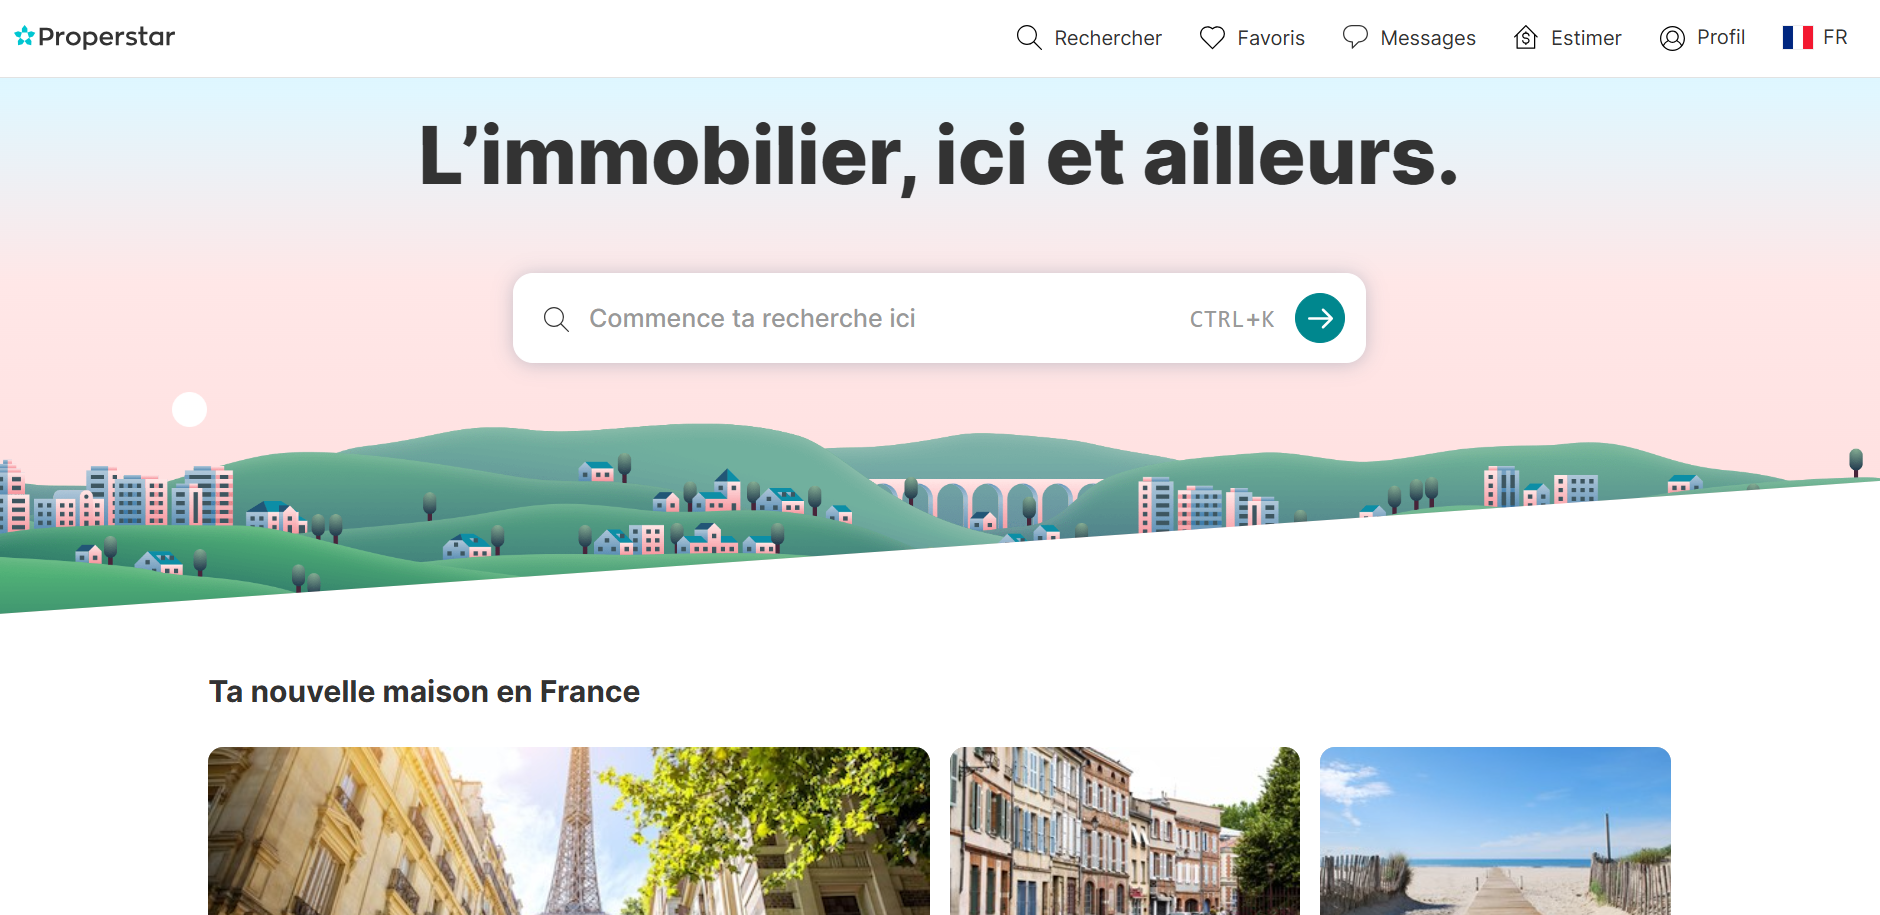
\includegraphics[width=\linewidth]{images/properstar.png}
        \caption{properstar website}
        \label{fig:properstar-website}
    \end{minipage}
    \hfill
    \begin{minipage}{0.47\textwidth}
        \centering
        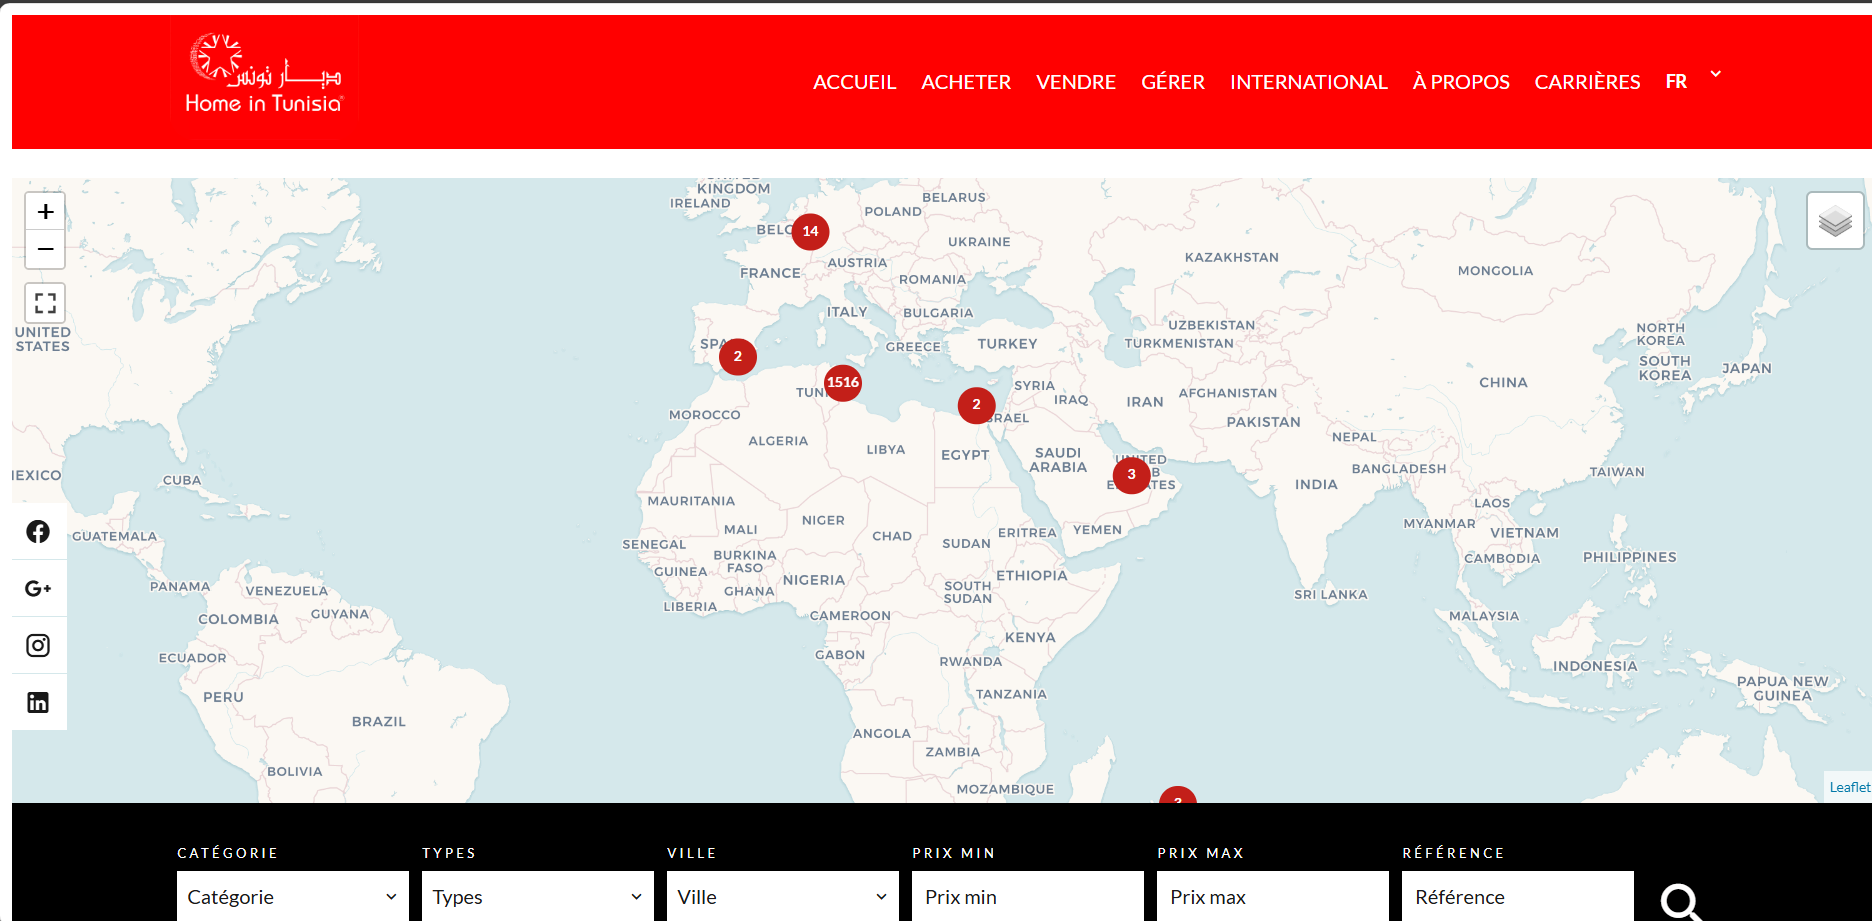
\includegraphics[width=\linewidth]{images/home_in_tunisia.png}
        \caption{homeintunisia website}
        \label{fig:homeintunisia-website}
    \end{minipage}
    
    \vspace{0.75cm}
    
    \begin{minipage}{0.47\textwidth}
        \centering
        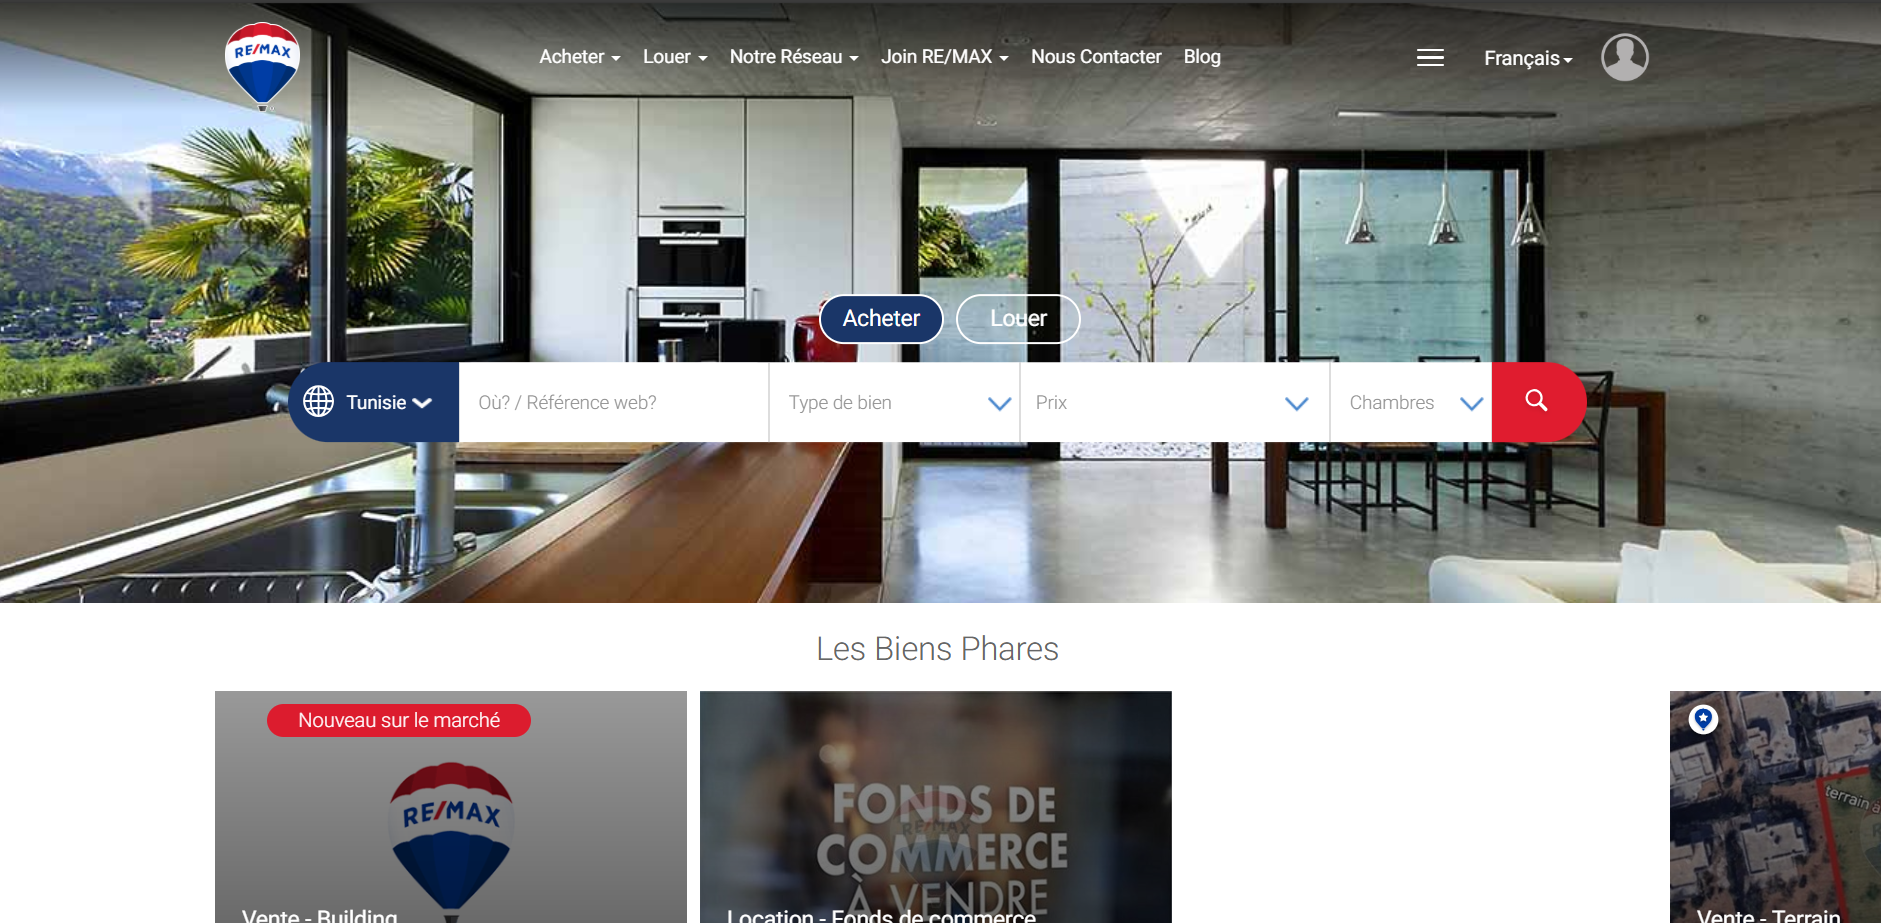
\includegraphics[width=\linewidth]{images/remax.png}
        \caption{remax website}
        \label{fig:remax-website}
    \end{minipage}
    \hfill
    \begin{minipage}{0.47\textwidth}
        \centering
        
\includegraphics[width=\linewidth]{images/mub.png}
        \caption{mubawab website}
        \label{fig:mubawab-website}
    \end{minipage}
\end{figure}

Our scraping system uses a distributed architecture with the following components:
\begin{itemize}
    \item Scheduled jobs for regular data updates, Data validation and cleaning pipelines
\end{itemize}

\begin{figure}[htbp]
    \centering
    % Placeholder for a diagram of the scraping workchart
    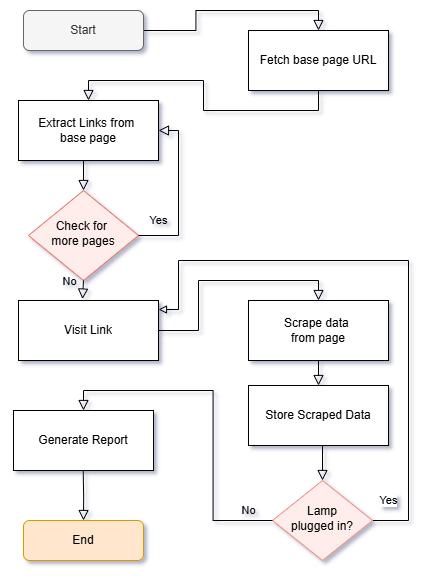
\includegraphics[width=0.35\textwidth]{images/workchartscraper.png}
    \caption{Data Scraping workchart}
    \label{fig:scraping-workchart}
\end{figure}

\newpage

\subsection{Implementation}
The data scraping system successfully collected comprehensive property information from multiple real estate platforms. Figure \ref{fig:scraping-output} demonstrates the structured output format of the scraped data, showing how property details are organized and stored for further processing by our AI models.
\begin{figure}[htbp]
    \centering
    % Top row - two images side by side
    \begin{minipage}{0.45\textwidth}
        \centering
        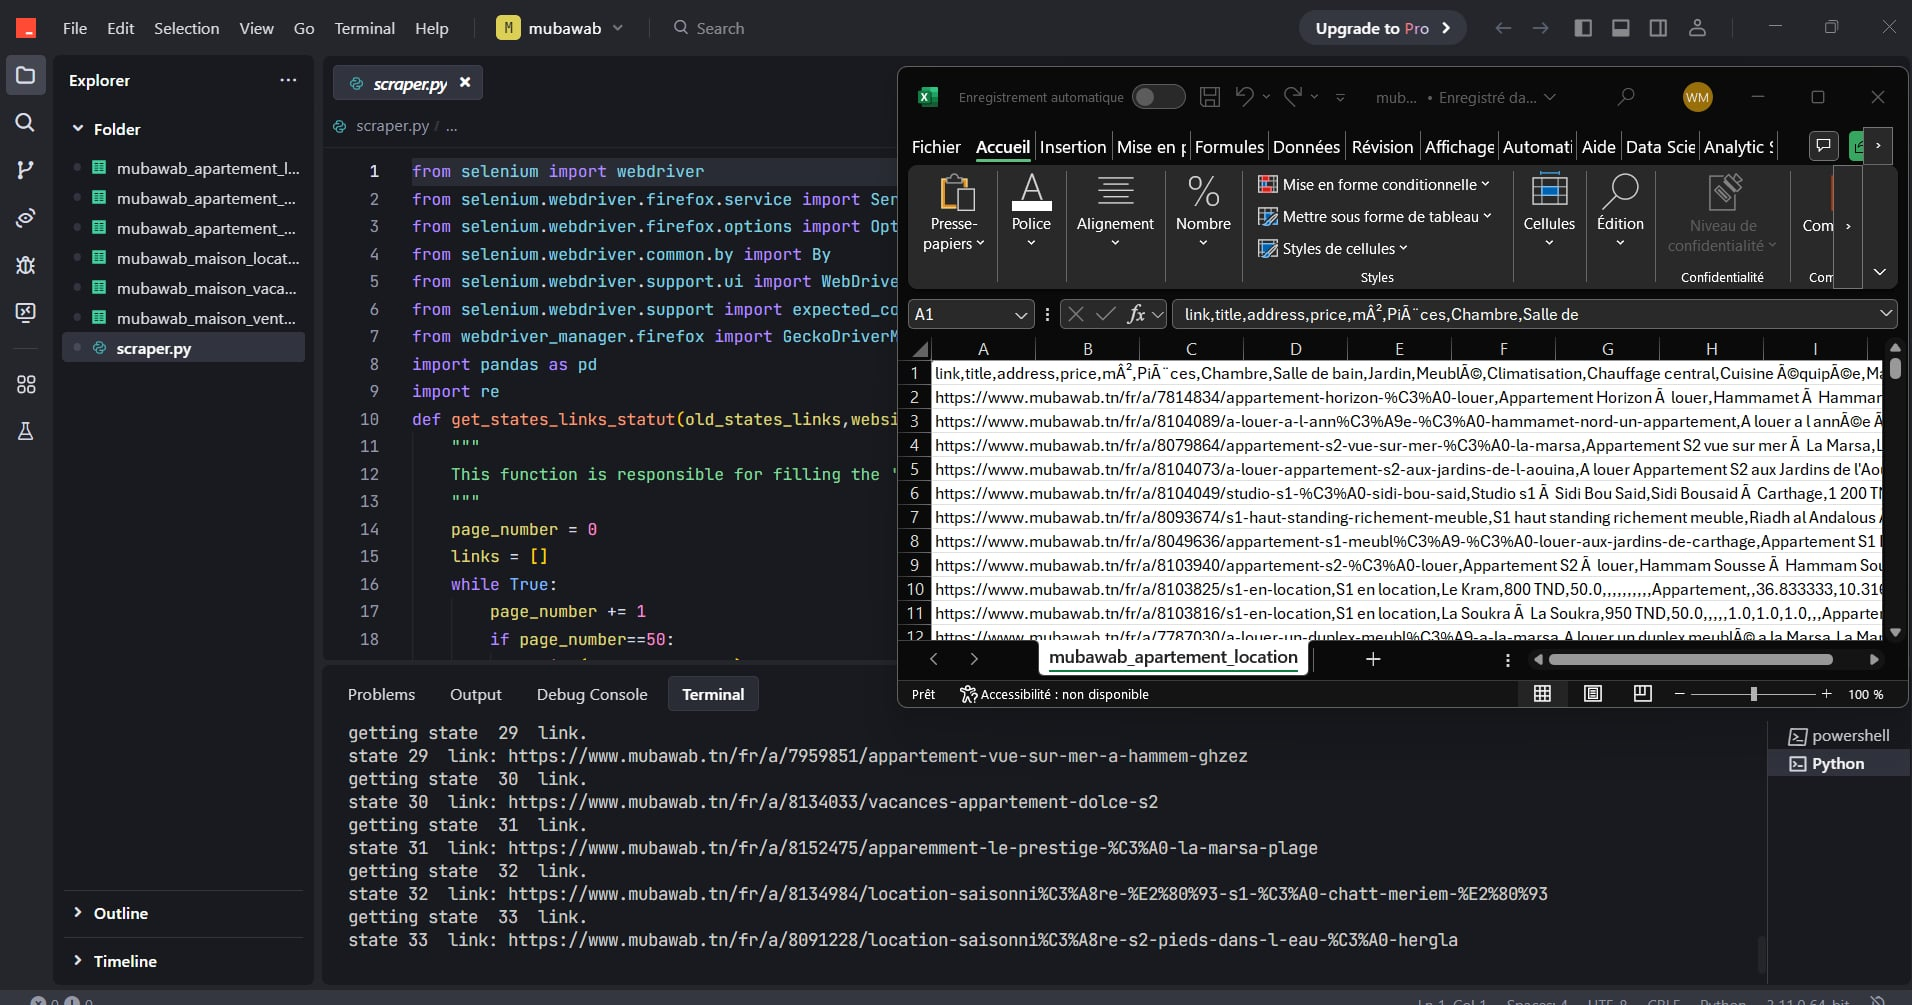
\includegraphics[width=\linewidth]{images/mubwab_scraper.jpeg}
        \caption*{Mubwab Scraper}
    \end{minipage}
    \hfill
    \begin{minipage}{0.45\textwidth}
        \centering
        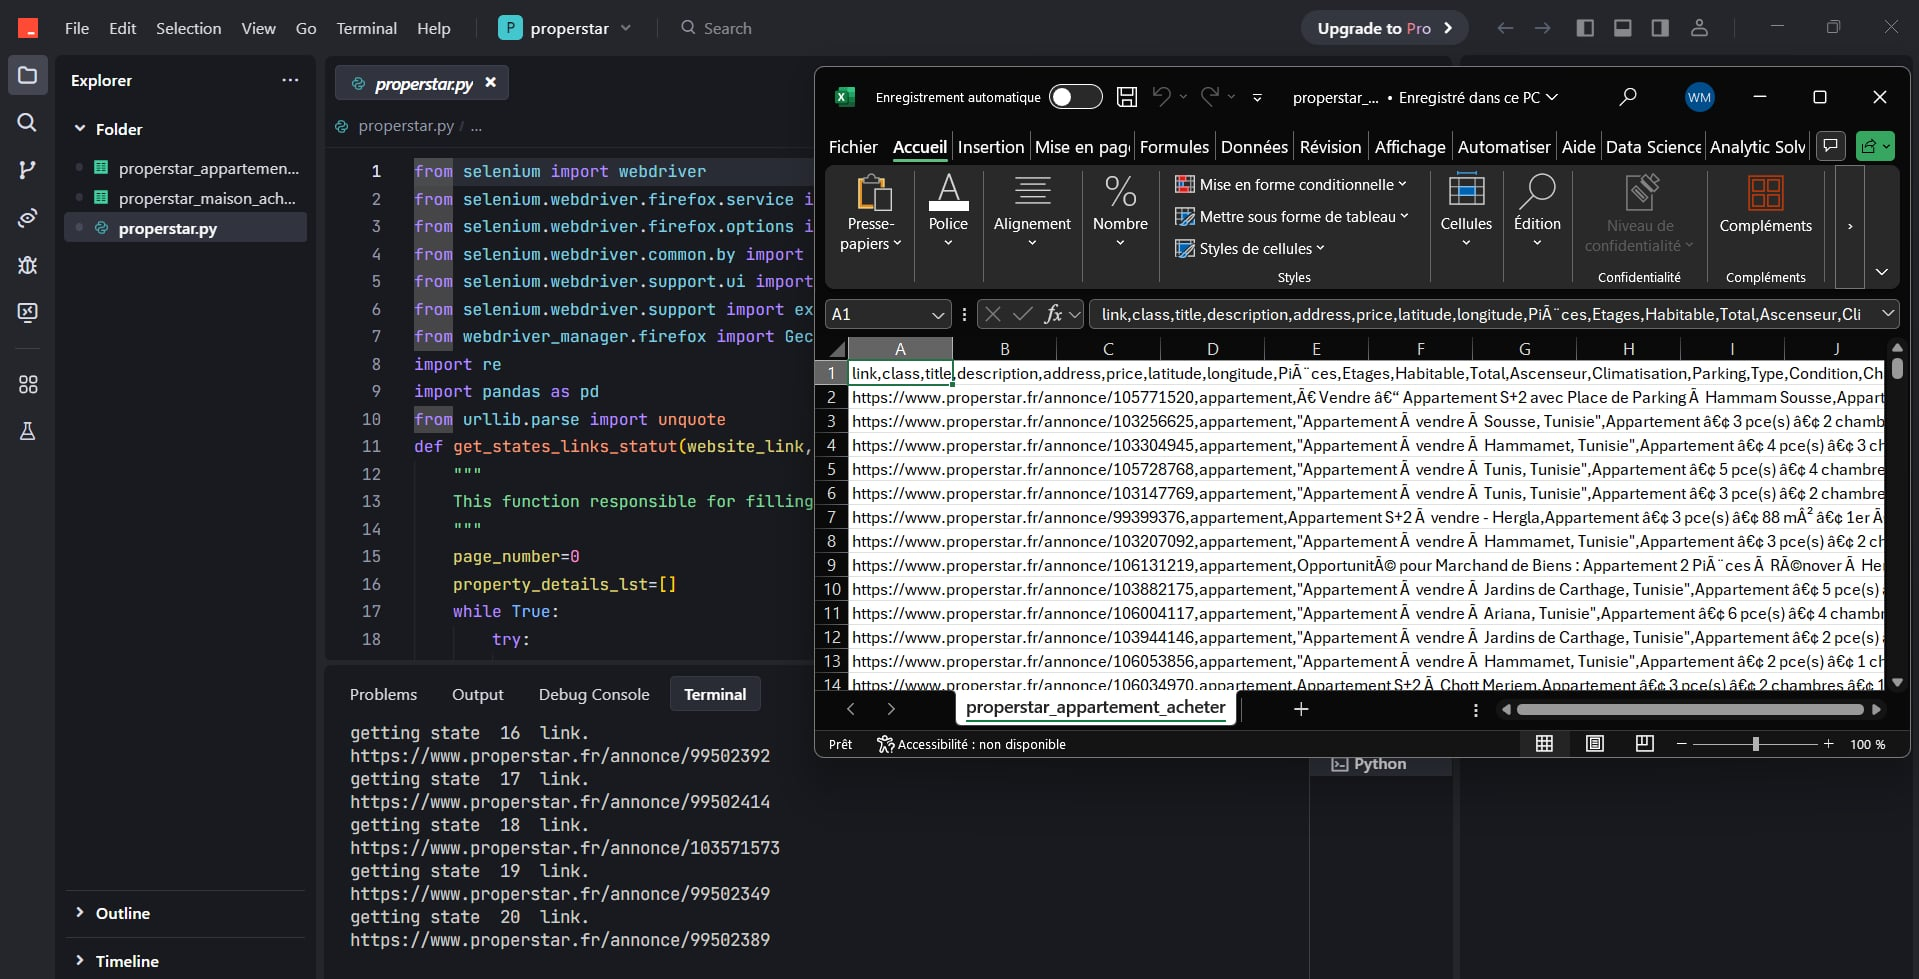
\includegraphics[width=\linewidth]{images/properstar_scraper.jpeg}
        \caption*{Properstar Scraper}
    \end{minipage}
    
    \vspace{1cm}
    
    % Bottom row - one centered image
    \begin{minipage}{0.5\textwidth}
        \centering
        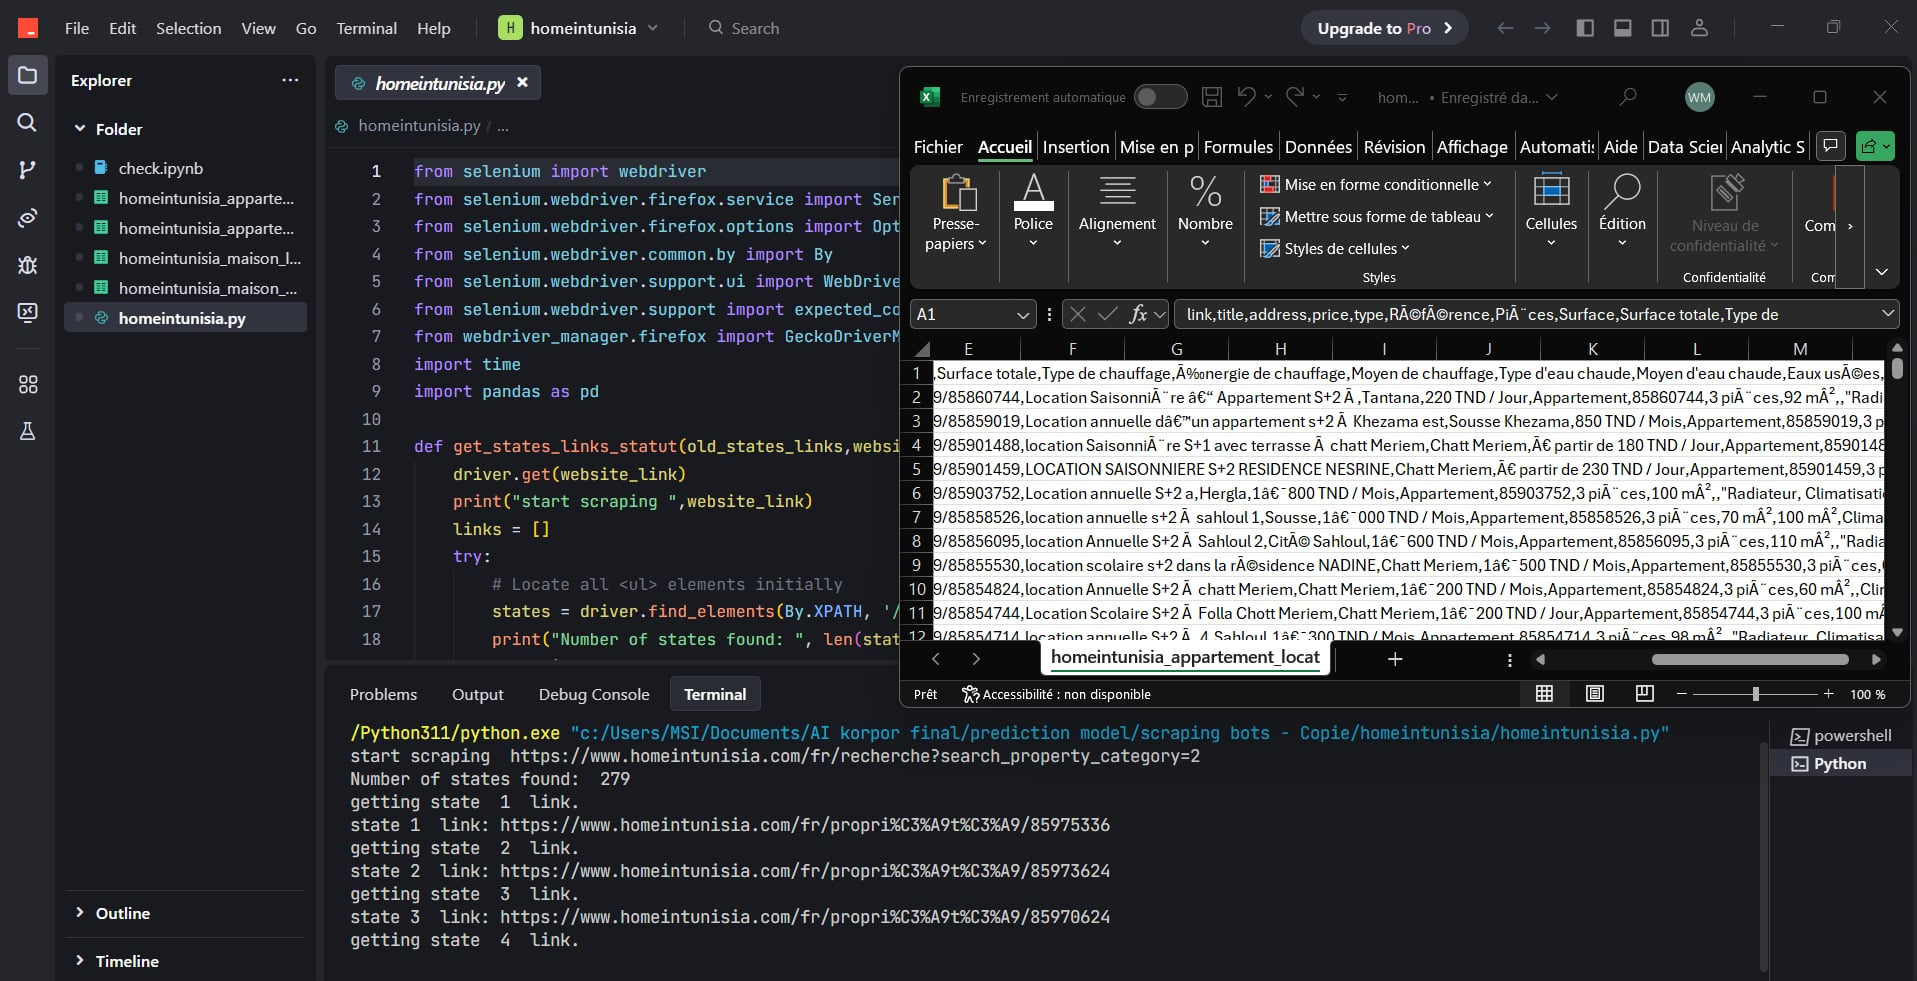
\includegraphics[width=\linewidth]{images/home_in_tunisia_scraper.jpeg}
        \caption*{Home in Tunisia Scraper}
    \end{minipage}
    \caption{Data Scraping Output Results}
    \label{fig:scraping-output}
\end{figure}

\newpage

\section{Sprint 3: Property Valuation Prediction Model}

\subsection*{Introduction}
The Property Valuation Prediction Model is designed to estimate both the market value and potential rental income for real estate properties. This provides investors with crucial information to make informed investment decisions.

\subsection{Analysis}
\subsubsection{Use Case Diagram}
The property valuation model serves multiple actors within the Korpor ecosystem. Figure \ref{fig:valuation-use-case} illustrates the primary use cases for the AI-powered property valuation system.
\begin{figure}[htbp]
    \centering
    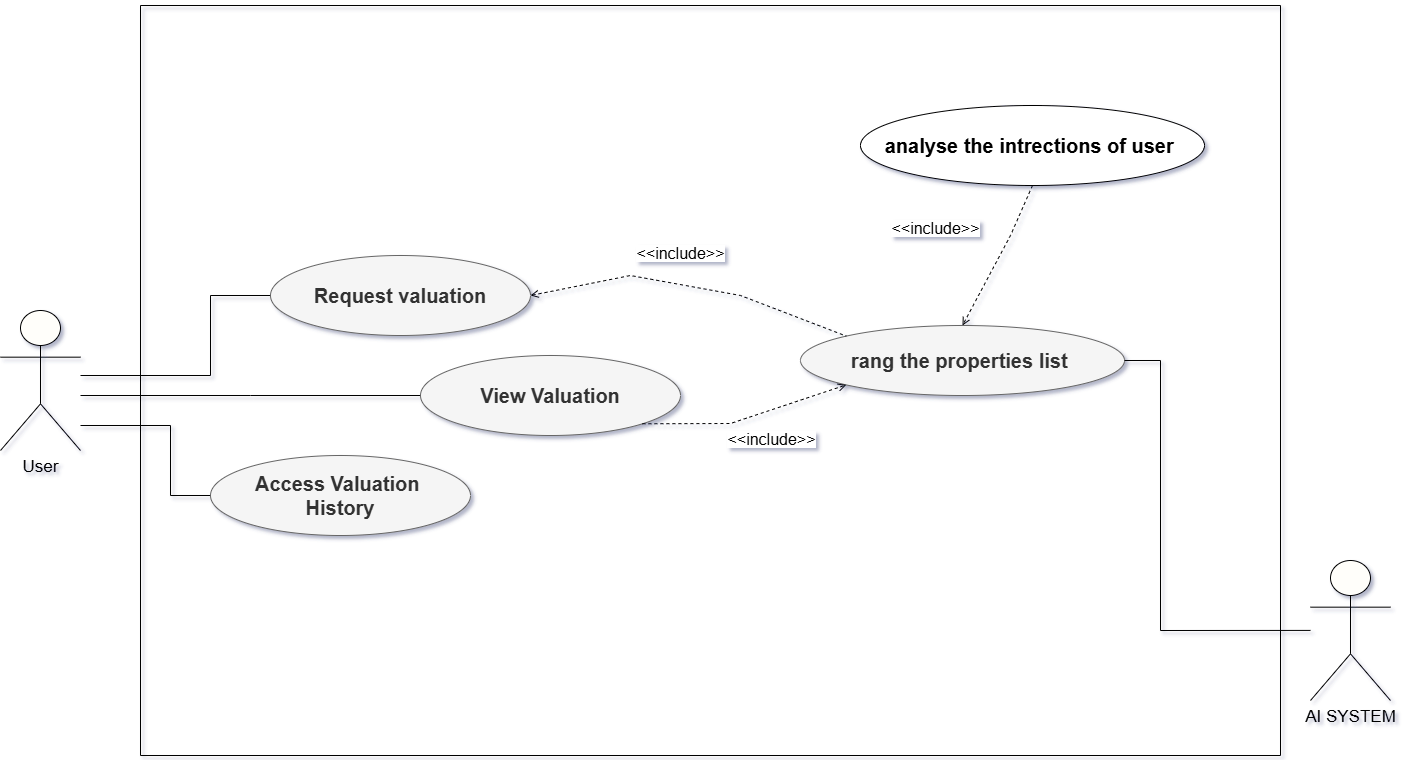
\includegraphics[width=0.8\textwidth]{images/valuation_use_case_diagram.png}
    \caption{Property Valuation Model Use Case Diagram}
    \label{fig:valuation-use-case}
\end{figure}

\subsubsection{Textual Use Case Descriptions}

\begin{table}[htbp]
    \centering
    \begin{tabular}{|p{3cm}|p{10cm}|}
        \hline
        \textbf{Use Case} & \textbf{Request Property Valuation} \\
        \hline
        \textbf{Actor} & User (representing Super Admin, Admin, Real Estate Agent) \\
        \hline
        \textbf{Precondition} & User is authenticated and has access to valuation features \\
        \hline
        \textbf{Main Scenario} & User gets market value and rental income predictions for a property \\
        \hline
        \textbf{Postcondition} & Valuation is stored and available for future reference \\
        \hline
    \end{tabular}
    \caption{Property Valuation Use Case Description}
    \label{tab:property-valuation-use-case}
\end{table}

\newpage

\subsection{Modeling}
\subsubsection{Class Diagram}
The property valuation system follows object-oriented design principles. Figure \ref{fig:valuation-class-diagram} shows the main classes and their relationships.

\begin{figure}[htbp]
    \centering
    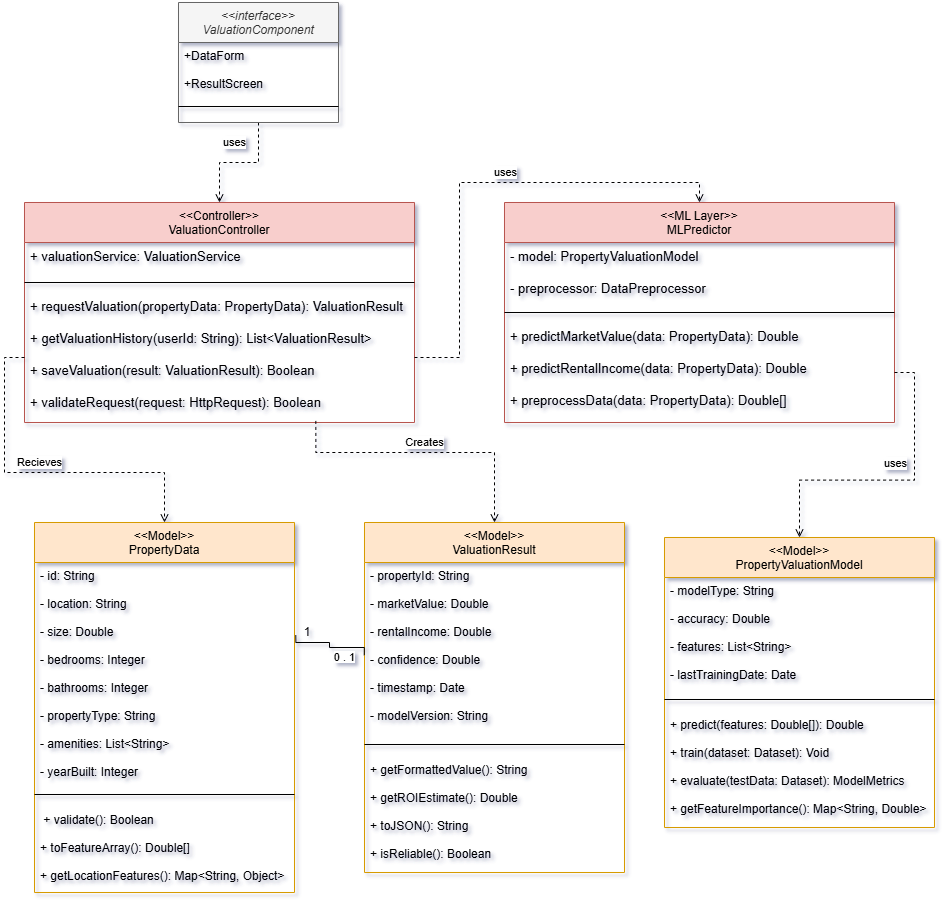
\includegraphics[width=1\textwidth]{images/valuation_class_diagram.png}
    \caption{Property Valuation Model Class Diagram}
    \label{fig:valuation-class-diagram}
\end{figure}

\newpage
The interaction sequence for the AI property valuation prediction model demonstrates the flow between different system components. Figure \ref{fig:ai-prediction-sequence-model} illustrates the sequence of operations from user request to prediction result delivery.

\begin{figure}[htbp]
    \centering
    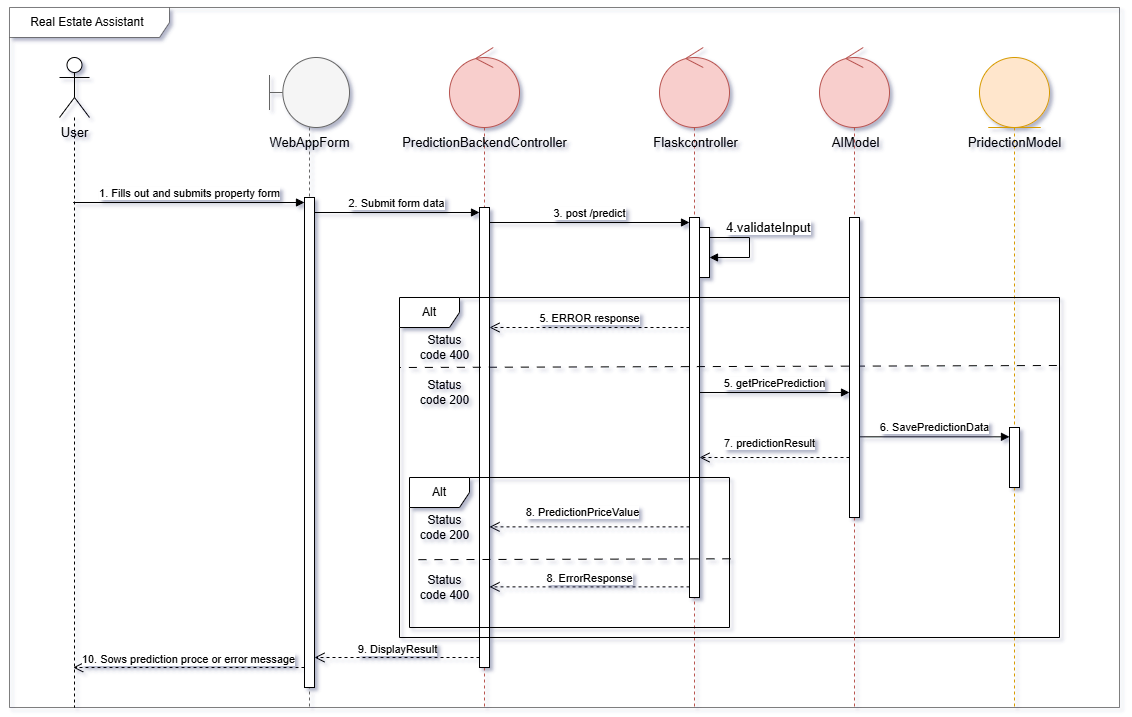
\includegraphics[width=1.1\textwidth]{images/sequence_AI_prediction_model.png}
    \caption{AI Property Valuation Prediction Sequence Diagram}
    \label{fig:ai-prediction-sequence-model}
\end{figure}

To provide a clearer understanding of the property valuation process, Figure \ref{fig:valuation-workflow} presents a simplified workflow diagram that illustrates the step-by-step flow from user input to prediction results.
\newpage
\begin{figure}[htbp]
    \centering
    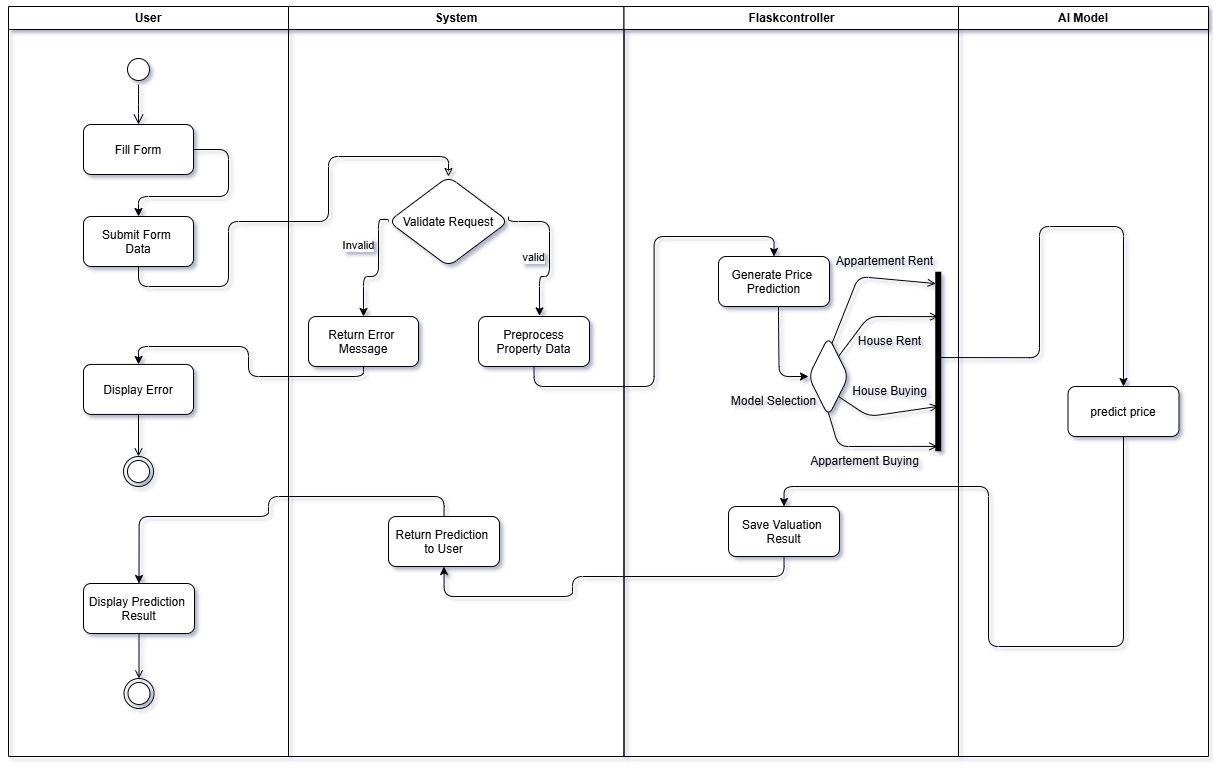
\includegraphics[width=1\textwidth]{images/valuation_workflow_diagram.png}
    \caption{Property Valuation Prediction Workflow Diagram}
    \label{fig:valuation-workflow}
\end{figure}

\subsection{Implementation}
\subsubsection{Data Features for Valuation}
The accuracy of the property valuation model heavily relies on the quality and comprehensiveness of the input data. Figure \ref{fig:geo-propriety-data} outlines the key geo-property data features utilized by the model. These features capture essential characteristics of a property and its location, enabling the model to learn complex relationships and predict market values and rental incomes effectively.
\newpage
\begin{figure}[htbp]
    \centering
    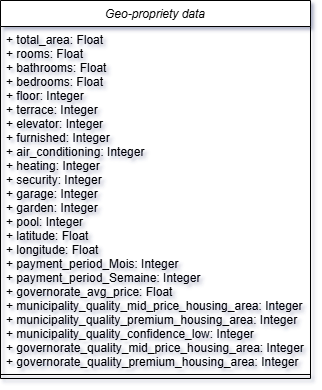
\includegraphics[width=0.4\textwidth]{images/geo-propriety-data.png} % Replace with your actual image path
    \caption{Geo-propriety Data Features for AI Models}
    \label{fig:geo-propriety-data}
\end{figure}

\subsubsection{Model Selection}
To develop an accurate property valuation prediction model, several regression algorithms were evaluated. The following models were selected for training and comparison due to their distinct characteristics and common effectiveness in similar predictive tasks:
\begin{itemize}
    \item \textbf{Linear Regression}: Chosen as a baseline model due to its simplicity and interpretability. It helps in understanding the linear relationships between the features and the target variables (market value and rental income).
    \item \textbf{Random Forest Regressor}: An ensemble learning method that operates by constructing a multitude of decision trees at training time. It is robust to overfitting, handles non-linear relationships well, and often provides high accuracy.
    \item \textbf{Gradient Boosting Regressor}: Another powerful ensemble technique that builds models in a stage-wise fashion. It is known for its high predictive accuracy and ability to optimize for various loss functions, making it suitable for complex regression tasks.
\end{itemize}
These models were trained on the prepared dataset, and their performances were evaluated to select the most suitable one for deployment in the Korpor platform.

\subsubsection{Feature Importance Analysis}
Understanding which features contribute most to the model's predictions is crucial for model interpretability and refinement. After training the selected model, a feature importance analysis was conducted. Figure \ref{fig:feature-importance} displays the top 15 most important features identified by the model. This analysis helps in validating the model's logic.
\newpage

\begin{figure}[htbp]
    \centering
    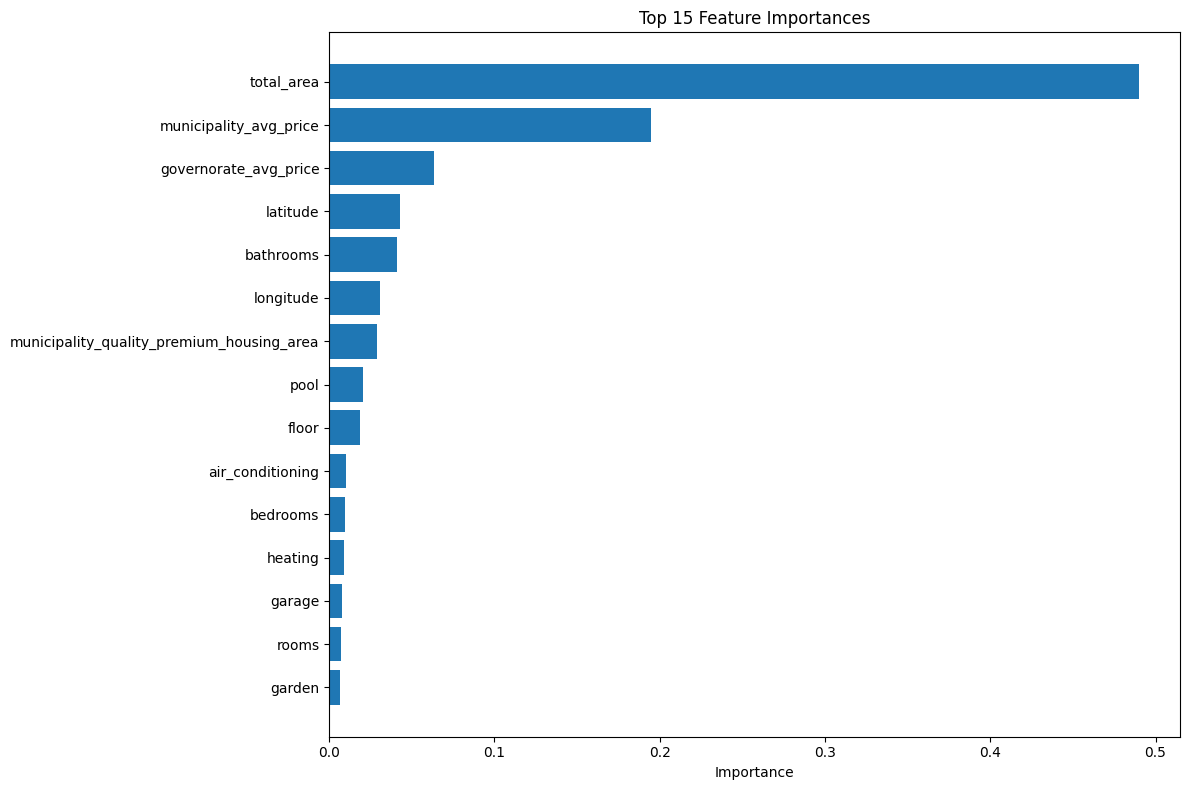
\includegraphics[width=0.8\textwidth]{images/top_15_feature_importance.png} % Assuming image is in 'images' directory
    \caption{Top 15 Feature Importance for Property Valuation Model}
    \label{fig:feature-importance}
\end{figure}

\subsubsection{Model Evaluation and Metrics}
The performance of the trained regression models was rigorously evaluated using standard metrics to ensure reliability and accuracy. Key metrics such as Mean Absolute Error (MAE), Mean Squared Error (MSE), Root Mean Squared Error (RMSE), and R-squared (R²) score were computed on a held-out test dataset. Figure \ref{fig:model-test-metrics} presents a summary of these performance metrics for the chosen valuation model. These results provide a quantitative assessment of the model's ability to generalize to unseen data.


\begin{figure}[htbp]
    \centering
    \begin{minipage}{0.48\textwidth}
        \centering
        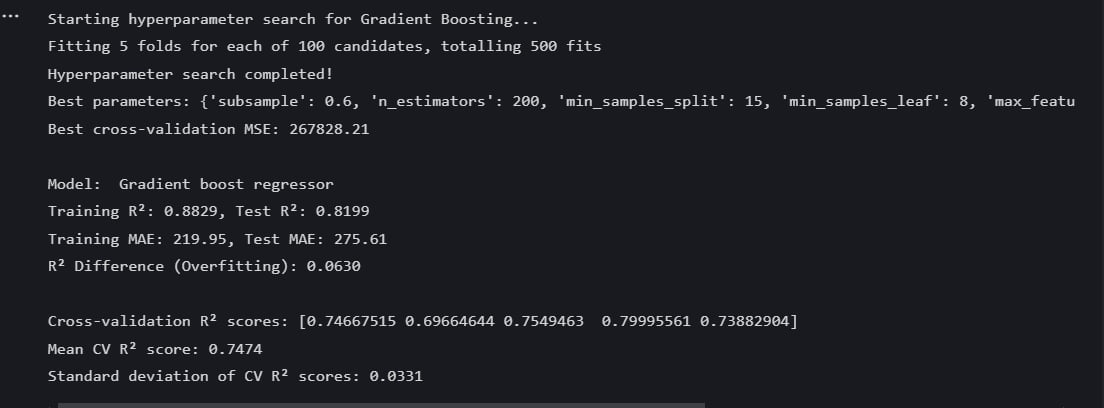
\includegraphics[width=\linewidth]{images/apartmenet location.jpeg}
        \caption*{Apartment Location Prediction}
    \end{minipage}
    \hfill
    \begin{minipage}{0.48\textwidth}
        \centering
        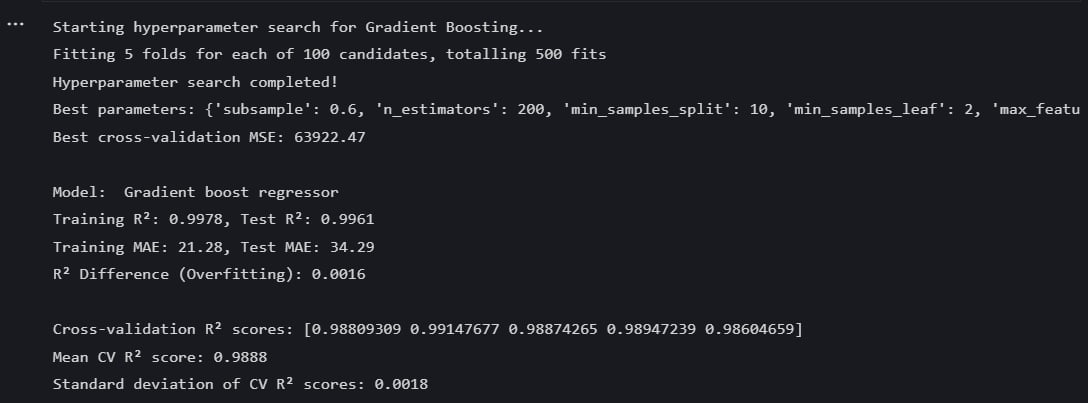
\includegraphics[width=\linewidth]{images/maison location.jpeg}
        \caption*{House Location Prediction}
    \end{minipage}
    
    \vspace{0.5cm}
    
    \begin{minipage}{0.48\textwidth}
        \centering
        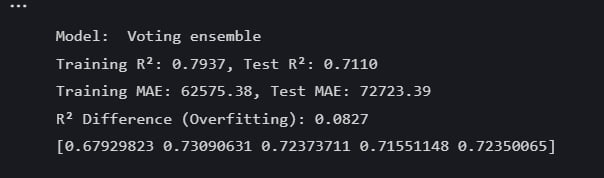
\includegraphics[width=\linewidth]{images/apartmeent vente.jpeg}
        \caption*{Apartment Sale Prediction}
    \end{minipage}
    \hfill
    \begin{minipage}{0.48\textwidth}
        \centering
        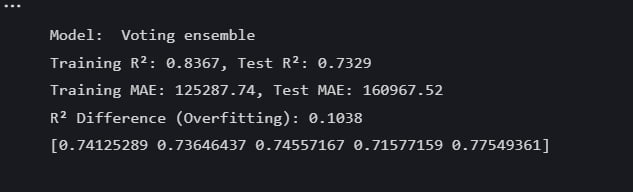
\includegraphics[width=\linewidth]{images/maison vente.jpeg}
        \caption*{House Sale Prediction}
    \end{minipage}
    
    \caption{Prediction Model Test Metrics Summary}
    \label{fig:model-test-metrics}
\end{figure}
\newpage

\subsubsection{Prediction User Interface}
Figure \ref{fig:prediction-form} shows the input form, and Figure \ref{fig:prediction-results} displays an example of the prediction results screen.

\begin{figure}[htbp]
        \centering
        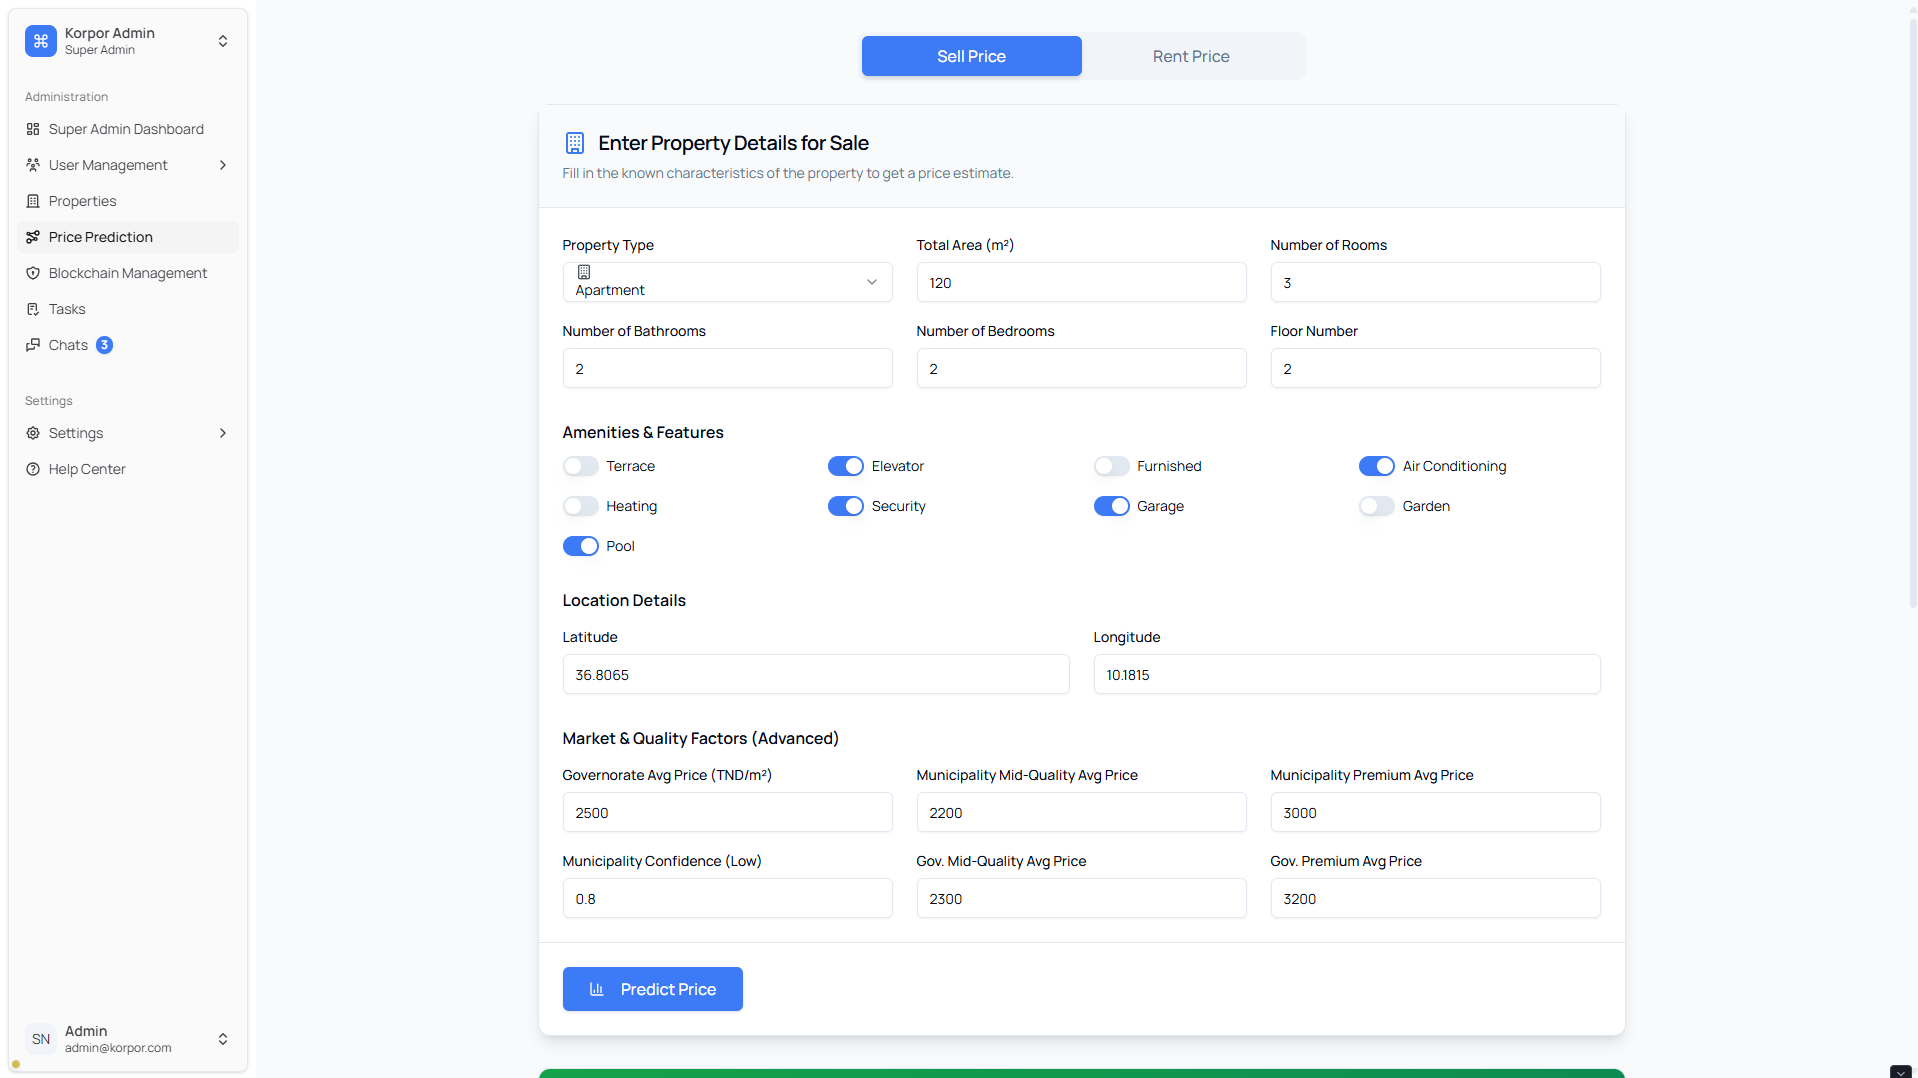
\includegraphics[width=0.7\textwidth]{images/screenshot_form_predition.png}
        \caption{Property Details Input Form for Valuation}
        \label{fig:prediction-form}
\end{figure}

\begin{figure}[htbp]
        \centering
        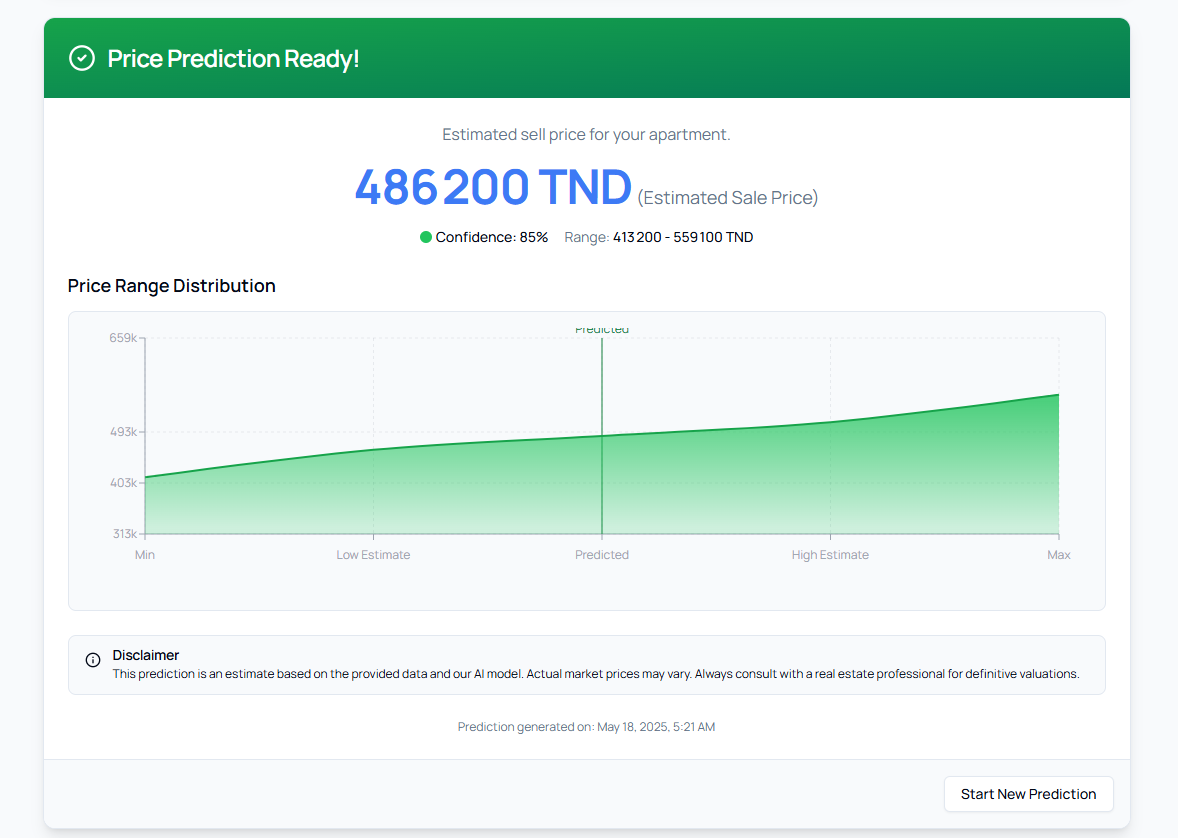
\includegraphics[width=0.7\textwidth]{images/screenshot_predctionscreen.png}
        \caption{Valuation Prediction Results Screen}
        \label{fig:prediction-results}
\end{figure}

\subsubsection{Mobile Investment Insights}
The Korpor mobile application provides investors with direct access to AI-powered property valuations, including future evaluation insights generated by the prediction model. This feature empowers users to make data-driven investment decisions by visualizing potential growth and returns. Figure \ref{fig:mobile-future-evaluation} showcases the mobile interface where these future evaluations are presented to the investor.
\newpage
\begin{figure}[htbp]
    \centering
    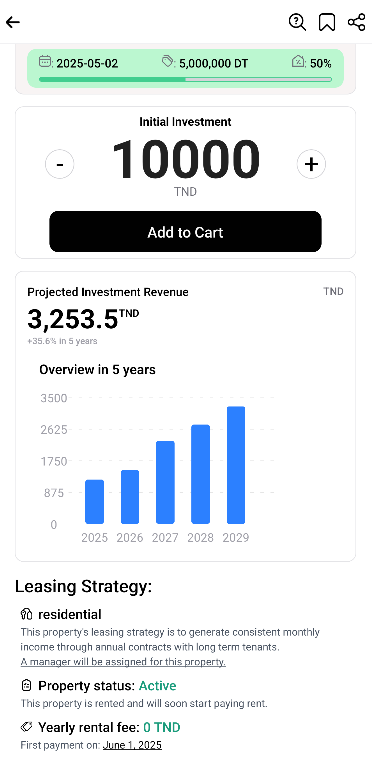
\includegraphics[width=0.3\textwidth]{images/mobile_future_evaluation.png} % Replace with your actual image path
    \caption{Mobile Interface for Future Property Evaluation Insights}
    \label{fig:mobile-future-evaluation}
\end{figure}


\subsection{Test}
\subsubsection{Mobile Interface Testing (Maestro)}
To ensure a seamless and reliable user experience on the mobile platform, the interface for displaying AI-driven property evaluations underwent end-to-end testing using Maestro. The tests covered user flows for accessing predictions and interacting with the displayed data. Figure \ref{fig:maestro-tests-mobile} shows the successful completion of these Maestro tests, validating the robustness of the mobile UI components related to the AI features.

\begin{figure}[htbp]
    \centering
    % \includegraphics[width=0.8\textwidth]{images/maestro_test_mobile_passed.png} % Replace with your actual image path
    \caption{Maestro Test Results for Mobile Prediction Interface}
    \label{fig:maestro-tests-mobile}
\end{figure}

\subsubsection{Model Performance Validation}
The property valuation model underwent comprehensive testing to ensure accuracy and reliability. The model achieved satisfactory performance metrics across different property types and locations, validating its effectiveness for real-world deployment.

\subsection{Retrospective}

The property valuation prediction model sprint provided valuable insights into AI model development and deployment. Table \ref{tab:valuation-retrospective} summarizes the key achievements, challenges, and lessons learned during this sprint.
\newpage
\begin{table}[htbp]
    \centering
    \begin{tabular}{|p{3cm}|p{10cm}|}
        \hline
        \textbf{Category} & \textbf{Details} \\
        \hline
        \textbf{What Went Well} & 
        \begin{itemize}
            \item Successfully implemented multiple regression algorithms
            \item Achieved good model performance metrics
            \item Feature importance analysis provided valuable insights
            \item Mobile interface integration worked seamlessly
            \item Comprehensive testing validated model reliability
        \end{itemize} \\
        \hline
        \textbf{Challenges} & 
        \begin{itemize}
            \item Data preprocessing required more time than anticipated
            \item Model hyperparameter tuning was computationally intensive
            \item Handling missing or incomplete property data
            \item Balancing model complexity with interpretability
        \end{itemize} \\
        \hline
    \end{tabular}
    \caption{Property Valuation Model Sprint Retrospective Summary}
    \label{tab:valuation-retrospective}
\end{table}

\newpage

\section{Sprint 4: Real Estate Assistant (NLP Chatbot)}
\subsection*{Introduction}
The Real Estate Assistant is an intelligent NLP-powered chatbot designed to provide investors with instant access to real estate legal information and guidance. This AI assistant helps users understand complex legal concepts, property regulations, and investment procedures through natural language conversations.

\subsection{Analysis}
\subsubsection{Use Case Diagram}
The Real Estate Assistant serves primarily investors who need legal guidance during their property investment journey. Figure \ref{fig:assistant-use-case} illustrates the main use cases for the AI assistant.
\begin{figure}[htbp]
    \centering
    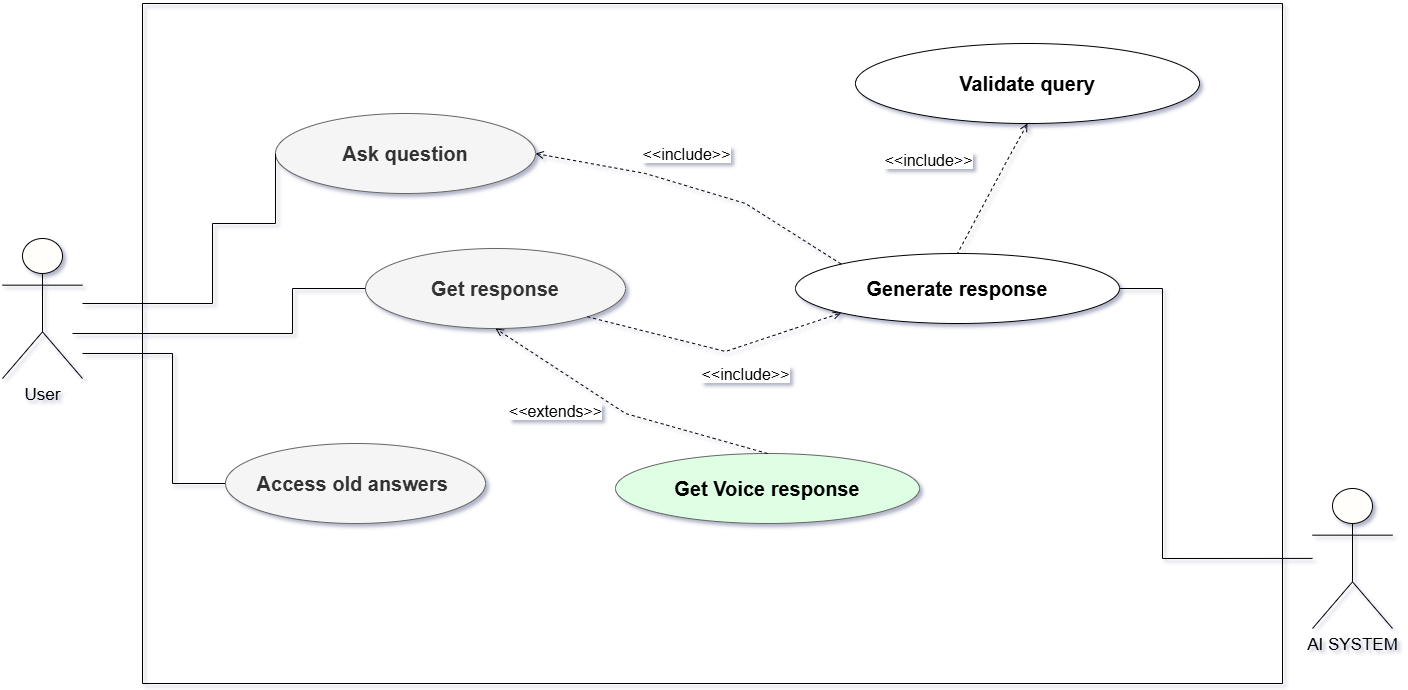
\includegraphics[width=0.9\textwidth]{images/assistant_use_case_diagram.png}
    \caption{Real Estate Assistant Use Case Diagram}
    \label{fig:assistant-use-case}
\end{figure}

\subsubsection{Textual Use Case Descriptions}

\begin{table}[htbp]
    \centering
    \begin{tabular}{|p{3cm}|p{10cm}|}
        \hline
        \textbf{Use Case} & \textbf{Ask Legal Question} \\
        \hline
        \textbf{Actor} & Investor \\
        \hline
        \textbf{Precondition} & User is authenticated and has access to the mobile app \\
        \hline
        \textbf{Main Scenario} & User get comprehensive answer \\
        \hline
        \textbf{Postcondition} & Conversation is saved for future reference \\
        \hline
    \end{tabular}
    \caption{Real Estate Assistant Use Case Description}
    \label{tab:assistant-use-case}
\end{table}

\newpage

\subsection{Modeling}
\subsubsection{Class Diagram}
The Real Estate Assistant follows a modular architecture for NLP processing and knowledge management. Figure \ref{fig:assistant-class-diagram} shows the main classes and their relationships.

\begin{figure}[htbp]
    \centering
    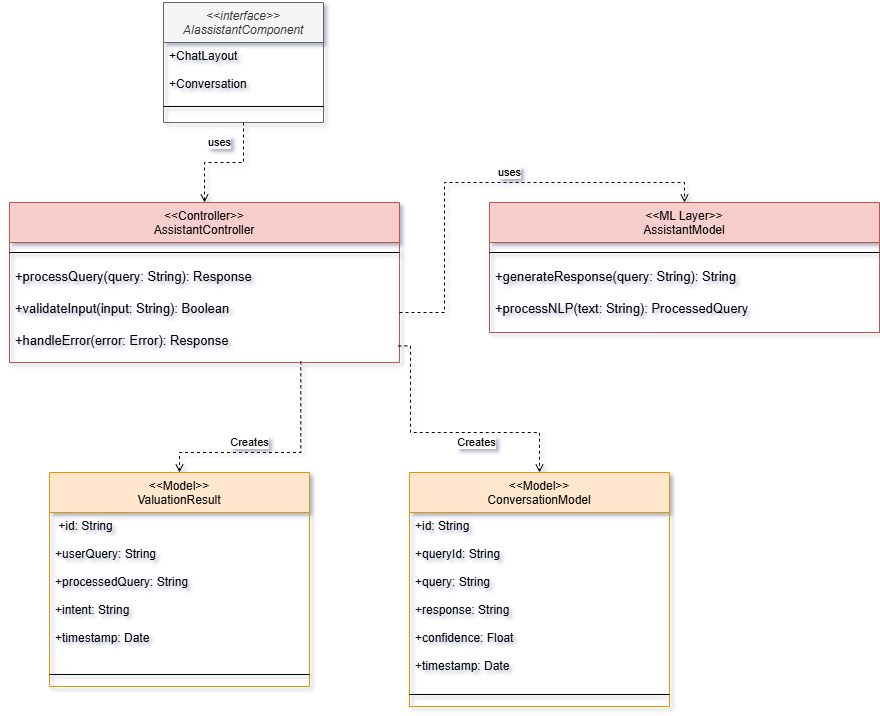
\includegraphics[width=0.9\textwidth]{images/assistant_class_diagram.png}
    \caption{Real Estate Assistant Class Diagram}
    \label{fig:assistant-class-diagram}
\end{figure}

\subsubsection{Sequence Diagram (MVC)}
The interaction flow between the mobile interface, backend services, and NLP processing components is illustrated in Figure \ref{fig:assistant-sequence-mvc}.
\newpage
\begin{figure}[htbp]
    \centering
    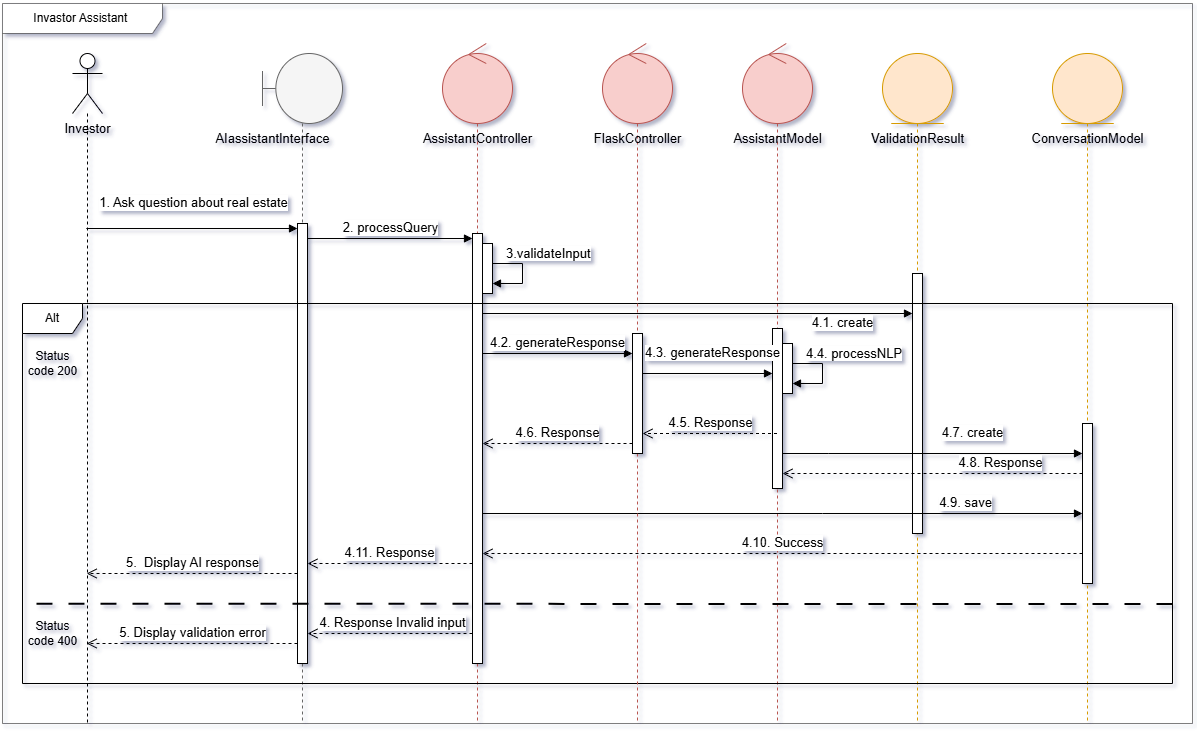
\includegraphics[width=1\textwidth]{images/assistant_sequence_mvc.png}
    \caption{Real Estate Assistant MVC Sequence Diagram}
    \label{fig:assistant-sequence-mvc}
\end{figure}

\subsubsection{Workflow Diagram}
The Real Estate Assistant follows a structured workflow to process user queries and provide accurate legal information. Figure \ref{fig:assistant-workflow} illustrates the complete workflow from user input to response generation.

\begin{figure}[htbp]
    \centering
    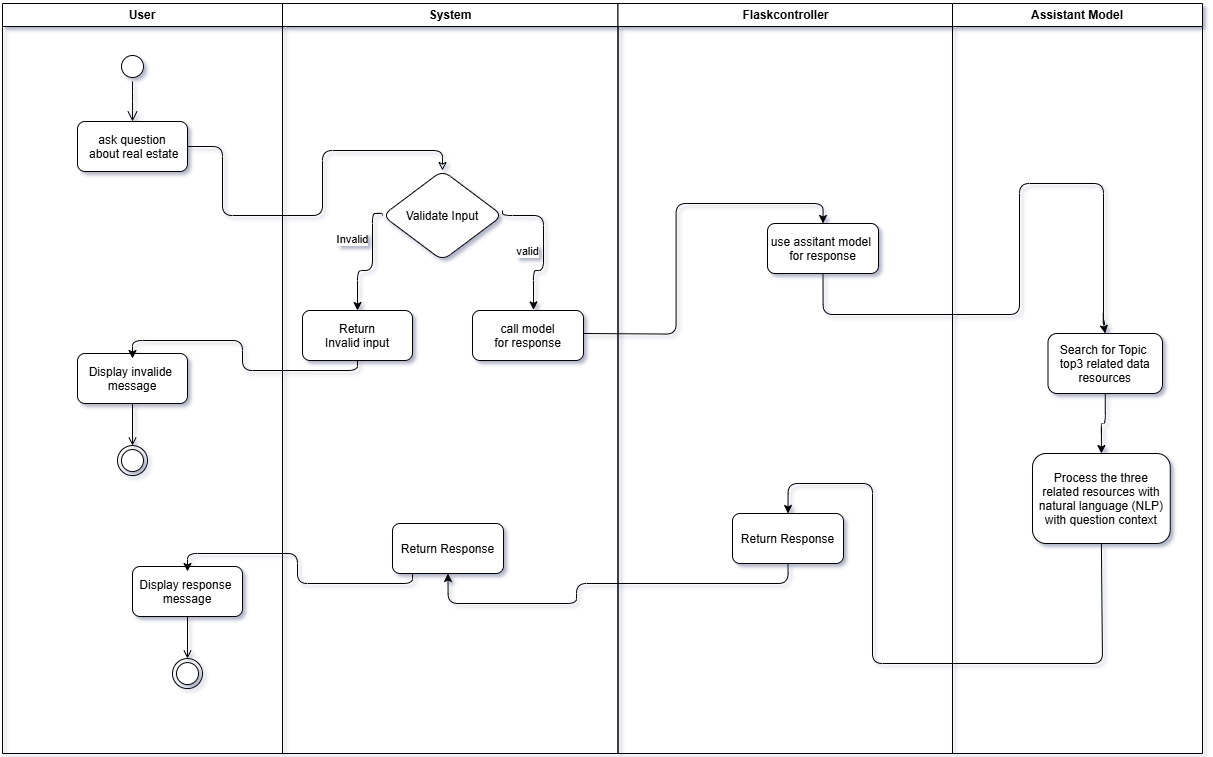
\includegraphics[width=0.9\textwidth]{images/assistant_workflow_diagram.png}
    \caption{Real Estate Assistant Workflow Diagram}
    \label{fig:assistant-workflow}
\end{figure}

\subsubsection{AI Approach Selection: RAG vs Fine-Tuning vs Prompt Engineering}

The development of the Real Estate Assistant required careful consideration of different AI approaches to ensure optimal performance for domain-specific legal and regulatory queries. This section analyzes the three primary approaches and justifies our selection.

\paragraph{Prompt Engineering}
Prompt engineering is the process of crafting input text (prompts) that guide a pre-trained language model to respond in a specific way. The purpose is to optimize the interaction between users and the model without modifying the underlying model parameters.

\textbf{Example Comparison:}
\begin{itemize}
    \item \textbf{Without prompt engineering:} User asks "What is the capital of France?" and receives a simple response: "Paris"
    \item \textbf{With prompt engineering:} The system uses a crafted prompt: "In a friendly tone, tell me: What is the capital of France?" resulting in: "Oh, that's easy! The capital of France is Paris!"
\end{itemize}

\paragraph{Fine-Tuning}
Fine-tuning involves training a pre-trained model using domain-specific datasets. While pre-trained models excel at general conversational abilities, they often struggle with specialized domains and may produce inaccurate responses or hallucinations when addressing intricate domain-specific questions.

\textbf{Characteristics:}
\begin{itemize}
    \item Requires substantial computational resources (high-end GPUs, large memory)
    \item Needs cleaned, labeled datasets specific to the domain
    \item Demands technical expertise in large language model training
    \item Suitable for specialized tasks with sufficient training data
\end{itemize}

\paragraph{Retrieval-Augmented Generation (RAG)}
RAG combines retrieval and generation components to make large language models context-aware using external data sources. The retriever fetches relevant information from knowledge bases or vector databases, which the generator then uses alongside the original query to produce accurate, contextually relevant responses.

\textbf{Conceptual Explanation:}
RAG is an AI architecture that enhances the capabilities of large language models by providing them with access to external knowledge sources. Unlike traditional language models that rely solely on their training data, RAG systems can dynamically retrieve and incorporate relevant information from external databases, documents, or knowledge bases to generate more accurate and contextually appropriate responses.

\textbf{Standard RAG Workflow:}
The RAG process follows a systematic four-step workflow:
\begin{enumerate}
    \item \textbf{Embed the user's query:} Convert the user's input into a vector representation that captures its semantic meaning
    \item \textbf{Retrieve relevant documents:} Search through the knowledge base using the query embedding to find the most relevant documents or passages
    \item \textbf{Add them into the model's prompt:} Combine the retrieved context with the original user query to create an enhanced prompt
    \item \textbf{Generate a response:} Use the LLM with this additional context to produce a comprehensive and accurate response
\end{enumerate}

\textbf{Embedding Concept:}
Embedding is a method of representing objects such as text, images, and audio as points in a continuous vector space where the locations of those points are semantically meaningful to machine learning algorithms. In the context of RAG, embeddings enable the system to understand and compare the semantic similarity between the user's query and the documents in the knowledge base, ensuring that the most relevant information is retrieved.

\begin{figure}[htbp]
    \centering
    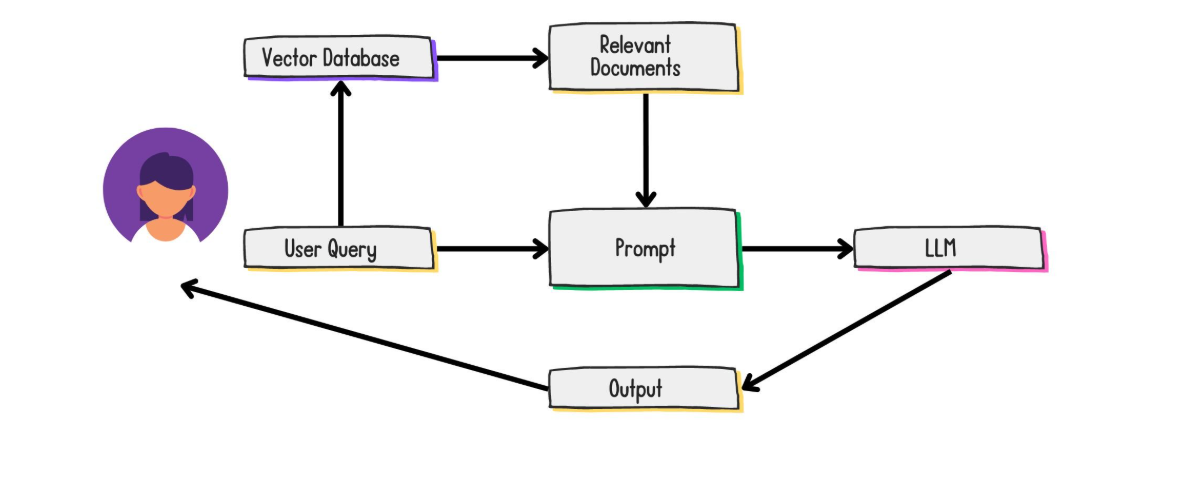
\includegraphics[width=0.9\textwidth]{images/rag_workflow_diagram.png}
    \caption{RAG Workflow Diagram}
    \label{fig:rag-workflow}
\end{figure}

\textbf{Advantages:}
\begin{itemize}
    \item Ideal for augmenting models with external, up-to-date, or domain-specific information
    \item Effective for constantly changing data (legal documents, regulations, FAQs)
    \item Requires limited resources and expertise compared to fine-tuning
    \item Can be implemented using established frameworks like LangChain and OpenAI API
\end{itemize}

\paragraph{Decision Rationale}
For our Real Estate Assistant, we selected RAG over the other approaches for the following reasons:

\begin{enumerate}
    \item \textbf{Domain Specificity:} Our model needs to respond using specialized knowledge about Tunisian real estate law and regulations that was not present in the pre-trained model's original training data
    \item \textbf{Resource Efficiency:} RAG implementation requires significantly fewer computational resources and technical expertise compared to fine-tuning
    \item \textbf{Data Characteristics:} Legal documents and regulations are constantly evolving, making RAG's ability to retrieve up-to-date information crucial
    \item \textbf{Development Speed:} RAG allows for rapid prototyping and deployment using existing frameworks and APIs
\end{enumerate}

Prompt engineering alone was insufficient for our use case, as we required the model to access and utilize domain-specific knowledge that extends beyond general conversational abilities.

\subsubsection{Prompt Engineering Implementation}
The following pseudo code demonstrates our prompt engineering approach for the Real Estate Assistant:

\begin{verbatim}
ALGORITHM: ChatPromptTemplate for Real Estate Assistant
INPUT: context, question, language
OUTPUT: structured_prompt

BEGIN
    // Initialize ChatPromptTemplate
    prompt = ChatPromptTemplate.from_template(
        "Based on the following context, provide a detailed answer to the user's query.
        
        Context: {context}
        User Query: {question}
        Response Language: {language}
        
        Instructions:
        1. Extract the relevant answer from the ANSWER section in the context
        2. Present the information in a clear, structured way
        3. Use the exact information from the context without adding external knowledge
        
        If the query is general conversation (like greetings, how are you, etc.), 
        respond naturally in the specified language.
        
        If the query is about a topic covered in the context but is within general knowledge, 
        respond with the exact information from context.
        
        If the query is not related to real estate, respond with the equivalent of 
        'I'm specialized in Tunisian real estate law and regulations.'
        
        If no relevant information is found and you cannot provide a general answer, 
        respond with the equivalent of 'I don't have specific information about this topic 
        in my current knowledge base.'"
    )
    
    // Format the prompt with actual values
    formatted_prompt = prompt.format(
        context=context,
        question=question,
        language=language
    )
    
    RETURN formatted_prompt
END
\end{verbatim}

\subsection{Implementation}

\subsubsection{Large Language Model Selection}
Choosing an appropriate LLM can be challenging given the numerous companies and different models available in the market. The host organization provided us with a Google Gemini API key, which constrained our selection to the available Gemini offerings.

Among the Gemini model family, we evaluated several options:
\begin{itemize}
    \item \textbf{Gemini 2.5 models}: While these represent the latest technology, they are still in experimental release phase, designed primarily to gather feedback and deliver updates quickly to developers
    \item \textbf{Gemini Flash 2.0}: Selected as the optimal choice based on efficiency and cost considerations
\end{itemize}

Gemini Flash 2.0 was chosen for the following reasons:
\begin{itemize}
    \item Superior efficiency and cost-effectiveness compared to other available models
    \item Lack of fine-tuning support, which reinforced our decision to implement RAG architecture
    \item Stable release status ensuring reliable performance for production deployment
\end{itemize}

\subsubsection{Voice Generation Implementation}
For voice generation capabilities, we selected ElevenLabs, an advanced AI-powered platform specializing in text-to-speech and voice synthesis technologies. ElevenLabs enables the generation of realistic, human-like voices suitable for various applications including narrations, audiobooks, podcasts, and video content.

The following pseudo code demonstrates our voice generation implementation:

\begin{verbatim}
ALGORITHM: Voice Generation for Real Estate Assistant
INPUT: text_response, user_preferences, voice_settings
OUTPUT: audio_stream

BEGIN
    // Initialize ElevenLabs API connection
    api_client = initialize_elevenlabs_client(API_KEY)
    
    // Voice configuration
    voice_id = get_selected_voice_id(user_preferences)
    voice_settings = {
        stability: 0.8,
    }
    
    // Text preprocessing
    cleaned_text = preprocess_text(text_response)
    chunks = split_text_into_chunks(cleaned_text, MAX_CHUNK_SIZE)
    
    // Voice generation process
    audio_segments = []
    FOR each chunk in chunks DO
        try:
            audio_segment = api_client.generate_voice(
                text=chunk,
                voice_id=voice_id,
                model="eleven_multilingual_v2",
                voice_settings=voice_settings
            )
            audio_segments.append(audio_segment)
        catch APIException as e:
            log_error("Voice generation failed: " + e.message)
            RETURN fallback_response()
        end try
    END FOR
    
    // Combine audio segments
    final_audio = concatenate_audio_segments(audio_segments)
    
    // Post-processing
    final_audio = apply_audio_filters(final_audio)
    final_audio = normalize_volume(final_audio)
    
    RETURN final_audio
END
\end{verbatim}


\subsubsection{NLP Model Architecture}
The Real Estate Assistant utilizes advanced natural language processing techniques to understand and respond to user queries. The system employs:

\begin{itemize}
    \item \textbf{Intent Recognition}: Identifies the purpose of user questions (property law, taxes, contracts, etc.)
    \item \textbf{Entity Extraction}: Extracts key information like property types, locations, and legal concepts
    \item \textbf{Context Management}: Maintains conversation history for coherent multi-turn dialogues
    \item \textbf{Response Generation}: Creates natural, informative responses based on legal knowledge base
\end{itemize}

\subsubsection{Legal Knowledge Base}
The assistant's knowledge base contains comprehensive information about:
\begin{itemize}
    \item Tunisian real estate law and regulations
    \item Property investment procedures
    \item Tax implications and calculations
    \item Contract templates and requirements
    \item Common legal issues and solutions
\end{itemize}

\subsubsection{Chat Interface Implementation}
The mobile chat interface provides an intuitive way for investors to interact with the AI assistant. Figure \ref{fig:assistant-mobile-chat} shows the chat interface design.
\newpage
\begin{figure}[htbp]
    \centering
    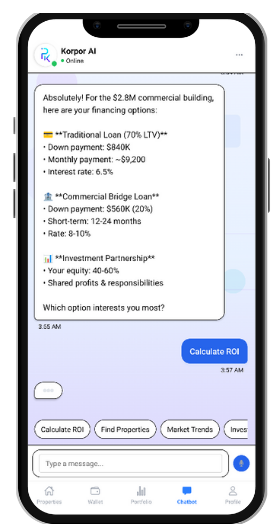
\includegraphics[width=0.3\textwidth]{images/assistant_mobile_chat.png}
    \caption{Mobile Chat Interface for Real Estate Assistant}
    \label{fig:assistant-mobile-chat}
\end{figure}


\subsection{Test}
\subsubsection{Test Scenarios}
The Real Estate Assistant underwent extensive testing to ensure accurate responses and reliable performance. Table \ref{tab:assistant-test-scenarios} presents the key test scenarios.

\begin{table}[htbp]
    \centering
    \begin{tabular}{|c|l|l|l|c|}
        \hline
        \textbf{Scenario} & \textbf{Input} & \textbf{Expected Output} & \textbf{Status} \\
        \hline
         Property tax query & "What are property taxes?" & Detailed tax information & \checkmark \\
        \hline
        Contract question & "What's in a rental contract?" & Contract requirements & \checkmark \\
        \hline
         Investment procedure & "How to buy property?" & Step-by-step guide & \checkmark \\
        \hline
         Legal compliance & "Foreign investment rules?" & Regulatory information & \checkmark \\
        \hline
         Context follow-up & Multi-turn conversation & Coherent responses & \checkmark \\
        \hline
         Unclear question & Ambiguous query & Clarification request & \checkmark \\
        \hline
    \end{tabular}
    \caption{Real Estate Assistant Test Scenarios}
    \label{tab:assistant-test-scenarios}
\end{table}

\newpage
\subsection{Retrospective}

The Real Estate Assistant sprint demonstrated the successful integration of NLP technology into the platform. Table \ref{tab:assistant-retrospective} summarizes the key outcomes and future improvements.

\begin{table}[htbp]
    \centering
    \begin{tabular}{|p{3cm}|p{10cm}|}
        \hline
        \textbf{Category} & \textbf{Details} \\
        \hline
        \textbf{What Went Well} & 
        \begin{itemize}
            \item Successfully implemented NLP chatbot functionality
            \item Mobile interface provides intuitive user experience
            \item Legal knowledge base effectively answers user queries
            \item Comprehensive testing validated system reliability
        \end{itemize} \\
        \hline
        \textbf{Action Items} & 
        \begin{itemize}
            \item Expand legal knowledge base coverage
            \item Implement multilingual support for broader accessibility
            \item Add conversation analytics for continuous improvement
            \item Integrate voice recognition capabilities
        \end{itemize} \\
        \hline
    \end{tabular}
    \caption{Real Estate Assistant Sprint Retrospective Summary}
    \label{tab:assistant-retrospective}
\end{table}

\newpage

\section{Sprint 5: Role-Based Backoffice Agent}
\subsection*{Introduction}
The Role-Based Backoffice Agent is an intelligent AI system designed to assist different user roles (Super Admin, Admin, Real Estate Agent) with automated task management, workflow optimization, and decision support. This AI agent adapts its behavior and recommendations based on the specific role and responsibilities of the authenticated user.

\subsection{Analysis}
\subsubsection{Use Case Diagram}
The Role-Based Backoffice Agent serves multiple user types with role-specific functionalities and automated assistance. Figure \ref{fig:backoffice-use-case} illustrates the main use cases for each role.

\begin{figure}[htbp]
    \centering
    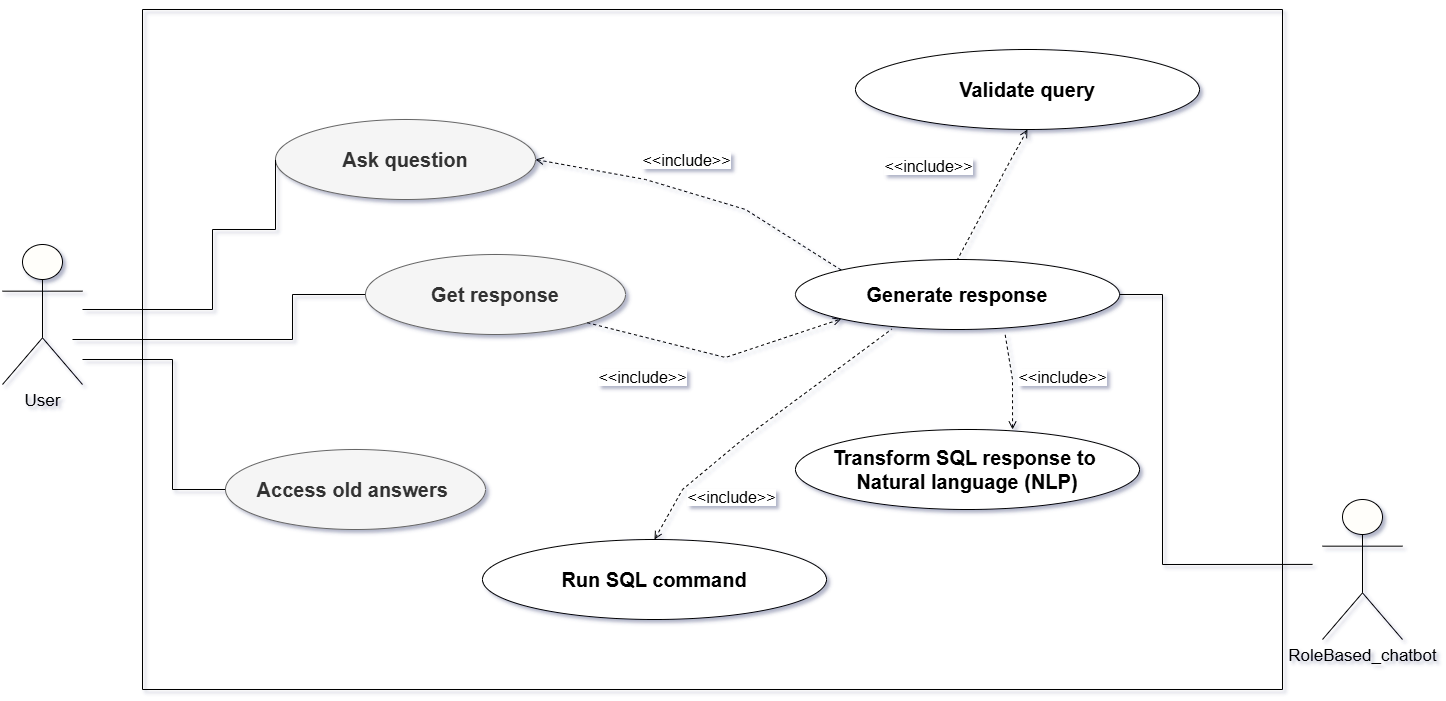
\includegraphics[width=1\textwidth]{images/backoffice_use_case_diagram.png}
    \caption{Role-Based Backoffice Agent Use Case Diagram}
    \label{fig:backoffice-use-case}
\end{figure}

\subsubsection{Textual Use Case Descriptions}

\begin{table}[htbp]
    \centering
    \begin{tabular}{|p{3cm}|p{10cm}|}
        \hline
        \textbf{Use Case} & \textbf{agent for administrative tasks} \\
        \hline
        \textbf{Actor} & User (representing Super Admin, Admin, Real Estate Agent) \\
        \hline
        \textbf{Precondition} & User is authenticated with specific role permissions \\
        \hline
        \textbf{Main Scenario} & User get comprehensive answer from platform database \\
        \hline
        \textbf{Postcondition} & Tasks are efficiently managed with minimal manual intervention \\
        \hline
    \end{tabular}
    \caption{Role-Based Backoffice Agent Use Case Description}
    \label{tab:backoffice-use-case}
\end{table}
\newpage

\subsection{Modeling}
\subsubsection{Class Diagram}
The Role-Based Backoffice Agent follows a role-based architecture with specialized services for each user type. Figure \ref{fig:backoffice-class-diagram} shows the main classes and their relationships.
\begin{figure}[htbp]
    \centering
    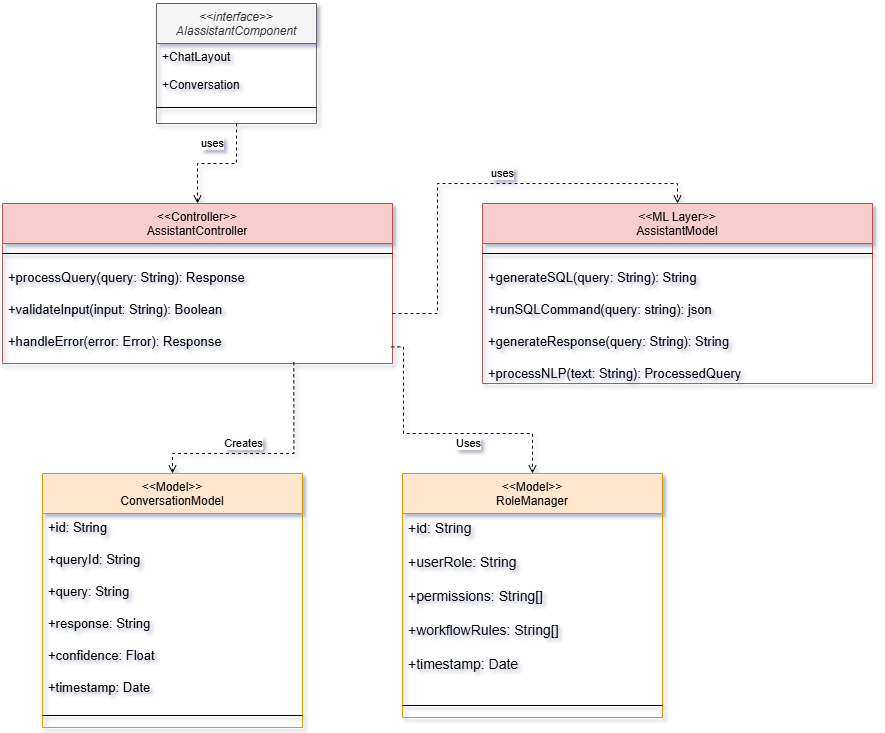
\includegraphics[width=1\textwidth]{images/backoffice_class_diagram.png}
    \caption{Role-Based Backoffice Agent Class Diagram}
    \label{fig:backoffice-class-diagram}
\end{figure}

\subsubsection{Sequence Diagram (MVC)}
The interaction flow between the web interface, role management services, and AI processing components is illustrated in Figure \ref{fig:backoffice-sequence-mvc}.
\newpage
\begin{figure}[htbp]
    \centering
    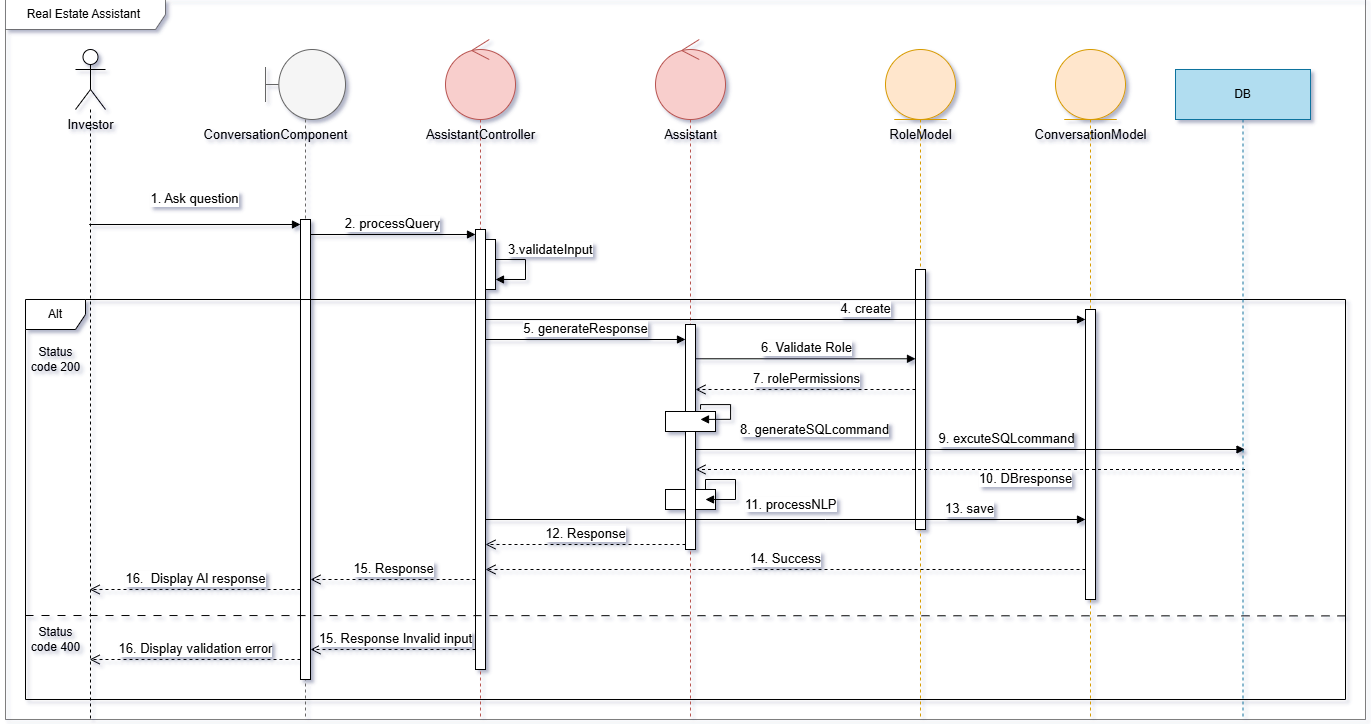
\includegraphics[width=1.1\textwidth]{images/backoffice_sequence_mvc.png}
    \caption{Role-Based Backoffice Agent MVC Sequence Diagram}
    \label{fig:backoffice-sequence-mvc}
\end{figure}

\subsection{Implementation}
\subsubsection{Role-Based AI Logic}
The Backoffice Agent utilizes sophisticated role-based AI algorithms to provide personalized assistance:

\begin{itemize}
    \item \textbf{Super Admin Features}: System monitoring, user management, platform analytics, security oversight
    \item \textbf{Admin Features}: Property management, user support, content moderation, performance tracking
    \item \textbf{Real Estate Agent Features}: Client management, property listings, sales tracking, commission calculations
\end{itemize}

\subsubsection*{Natural Language to SQL Processing}
The following pseudo code demonstrates the complete workflow for converting natural language queries to SQL and generating human-readable responses:

\paragraph{Natural Language to SQL Generation}
\begin{verbatim}
FUNCTION convert_question_to_sql(user_question, user_id):
    
    // Step 1: Get user information
    user_info = get_user_role_and_store(user_id)
    role = user_info.role          // 'user', 'admin', or 'super_admin'
    store_id = user_info.store_id
    
    // Step 2: Create database description with permissions
    database_info = build_database_description(role, store_id)
    
    // Step 3: Ask AI to write SQL
    prompt = "Given this database: {database_info}
              User asks: {user_question}
              Write a MySQL query that respects user permissions.
              Only return the SQL code."
    
    sql_query = ask_ai_model(prompt)
    clean_sql = remove_formatting(sql_query)
    
    // Step 4: Check if SQL is safe
    IF is_sql_safe(clean_sql, role, store_id):
        RETURN clean_sql
    ELSE:
        RETURN "Cannot create safe query"

FUNCTION get_user_role_and_store(user_id):
    query = "SELECT role, store_id FROM users WHERE id = ?"
    result = execute_database_query(query, user_id)
    RETURN result

FUNCTION build_database_description(role, store_id):
    description = "Tables: users, properties, stores, transactions, clients
                   
                   Access Rules:
                   - user: Can only see their store's data
                   - admin: Can see all data in their store  
                   - super_admin: Can see everything"
    
    IF role != 'super_admin':
        description += f"IMPORTANT: Must filter by store_id = {store_id}"
    
    RETURN description

FUNCTION is_sql_safe(sql, role, store_id):
    // Block dangerous operations
    dangerous_words = ['DELETE', 'DROP', 'UPDATE', 'INSERT']
    FOR word IN dangerous_words:
        IF word IN sql.upper():
            RETURN false
    
    // Check role permissions
    IF role != 'super_admin' AND 'WHERE' NOT IN sql.upper():
        RETURN false  // Must have WHERE clause
    
    RETURN true
\end{verbatim}

\paragraph{SQL Query Execution}
\begin{verbatim}
FUNCTION run_sql_query(sql_query):
    
    TRY:
        // Step 1: Connect to database
        connection = connect_to_database()
        
        // Step 2: Run the query with timeout
        start_time = current_time()
        results = execute_query(connection, sql_query, timeout=30)
        end_time = current_time()
        
        // Step 3: Limit results if too many
        IF length(results) > 1000:
            results = first_1000_items(results)
            results.add("... (truncated)")
        
        // Step 4: Return success
        RETURN {
            'success': true,
            'data': results,
            'execution_time': end_time - start_time
        }
    
    CATCH error:
        // Step 5: Handle errors nicely
        user_message = make_error_friendly(error)
        RETURN {
            'success': false,
            'error': user_message
        }
    
    FINALLY:
        close_database_connection(connection)

FUNCTION make_error_friendly(database_error):
    error_text = string(database_error).lower()
    
    IF 'syntax' IN error_text:
        RETURN "There's a problem with the query format"
    ELSE IF 'timeout' IN error_text:
        RETURN "Query took too long to run"
    ELSE IF 'connection' IN error_text:
        RETURN "Cannot connect to database"
    ELSE:
        RETURN "Database error occurred"
\end{verbatim}

\paragraph{Database Results to Natural Language}
\begin{verbatim}
FUNCTION convert_results_to_answer(query_results, user_role):
    
    // Step 1: Check if we have data
    IF query_results is empty:
        RETURN "No data found for your request"
    
    // Step 2: Choose response style based on user role
    response_style = get_response_style(user_role)
    
    // Step 3: Prepare data for AI
    simplified_data = simplify_data_for_ai(query_results)
    
    // Step 4: Ask AI to write natural response
    prompt = f"Convert this data to natural language:
              Data: {simplified_data}
              Style: {response_style}
              Keep it short and clear."
    
    natural_response = ask_ai_model(prompt)
    clean_response = clean_ai_response(natural_response)
    
    RETURN clean_response

FUNCTION get_response_style(user_role):
    styles = {
        'super_admin': "Executive summary with key insights",
        'admin': "Management report with important numbers", 
        'user': "Simple explanation in everyday language"
    }
    RETURN styles[user_role]

FUNCTION simplify_data_for_ai(results):
    // If too much data, summarize it
    IF length(results) > 50:
        summary = create_data_summary(results)
        RETURN summary
    ELSE:
        RETURN results

FUNCTION create_data_summary(large_dataset):
    summary = {
        'total_rows': length(large_dataset),
        'sample_data': first_10_rows(large_dataset),
        'key_numbers': extract_important_numbers(large_dataset)
    }
    RETURN summary
\end{verbatim}

\paragraph{Main Processing Flow}
\begin{verbatim}
FUNCTION process_user_request(user_question, user_id):
    
    // Step 1: Convert question to SQL
    sql_query = convert_question_to_sql(user_question, user_id)
    
    IF sql_query == "Cannot create safe query":
        RETURN "Sorry, I cannot process that request safely"
    
    // Step 2: Run the SQL query
    query_results = run_sql_query(sql_query)
    
    IF query_results.success == false:
        RETURN f"Database error: {query_results.error}"
    
    // Step 3: Convert results to natural language
    user_info = get_user_role_and_store(user_id)
    final_answer = convert_results_to_answer(query_results.data, user_info.role)
    
    // Step 4: Log the interaction (optional)
    log_interaction(user_question, sql_query, final_answer, user_id)
    
    RETURN final_answer

// Example usage
FUNCTION main():
    user_question = "How many properties do we have listed?"
    user_id = 3
    
    answer = process_user_request(user_question, user_id)
    print(answer)
\end{verbatim}

\subsubsection{Automated Workflow Management}
The system automates routine tasks based on role permissions:
\begin{itemize}
    \item Property approval workflows for admins
    \item User verification processes for super admins
    \item Client follow-up reminders for agents
    \item Performance report generation for all roles
\end{itemize}

\subsubsection{Dashboard Implementation}
Each role receives a customized dashboard with relevant tools and insights. Figure \ref{fig:backoffice-dashboard} shows the role-specific dashboard implementations.

\begin{figure}[htbp]
    \centering
    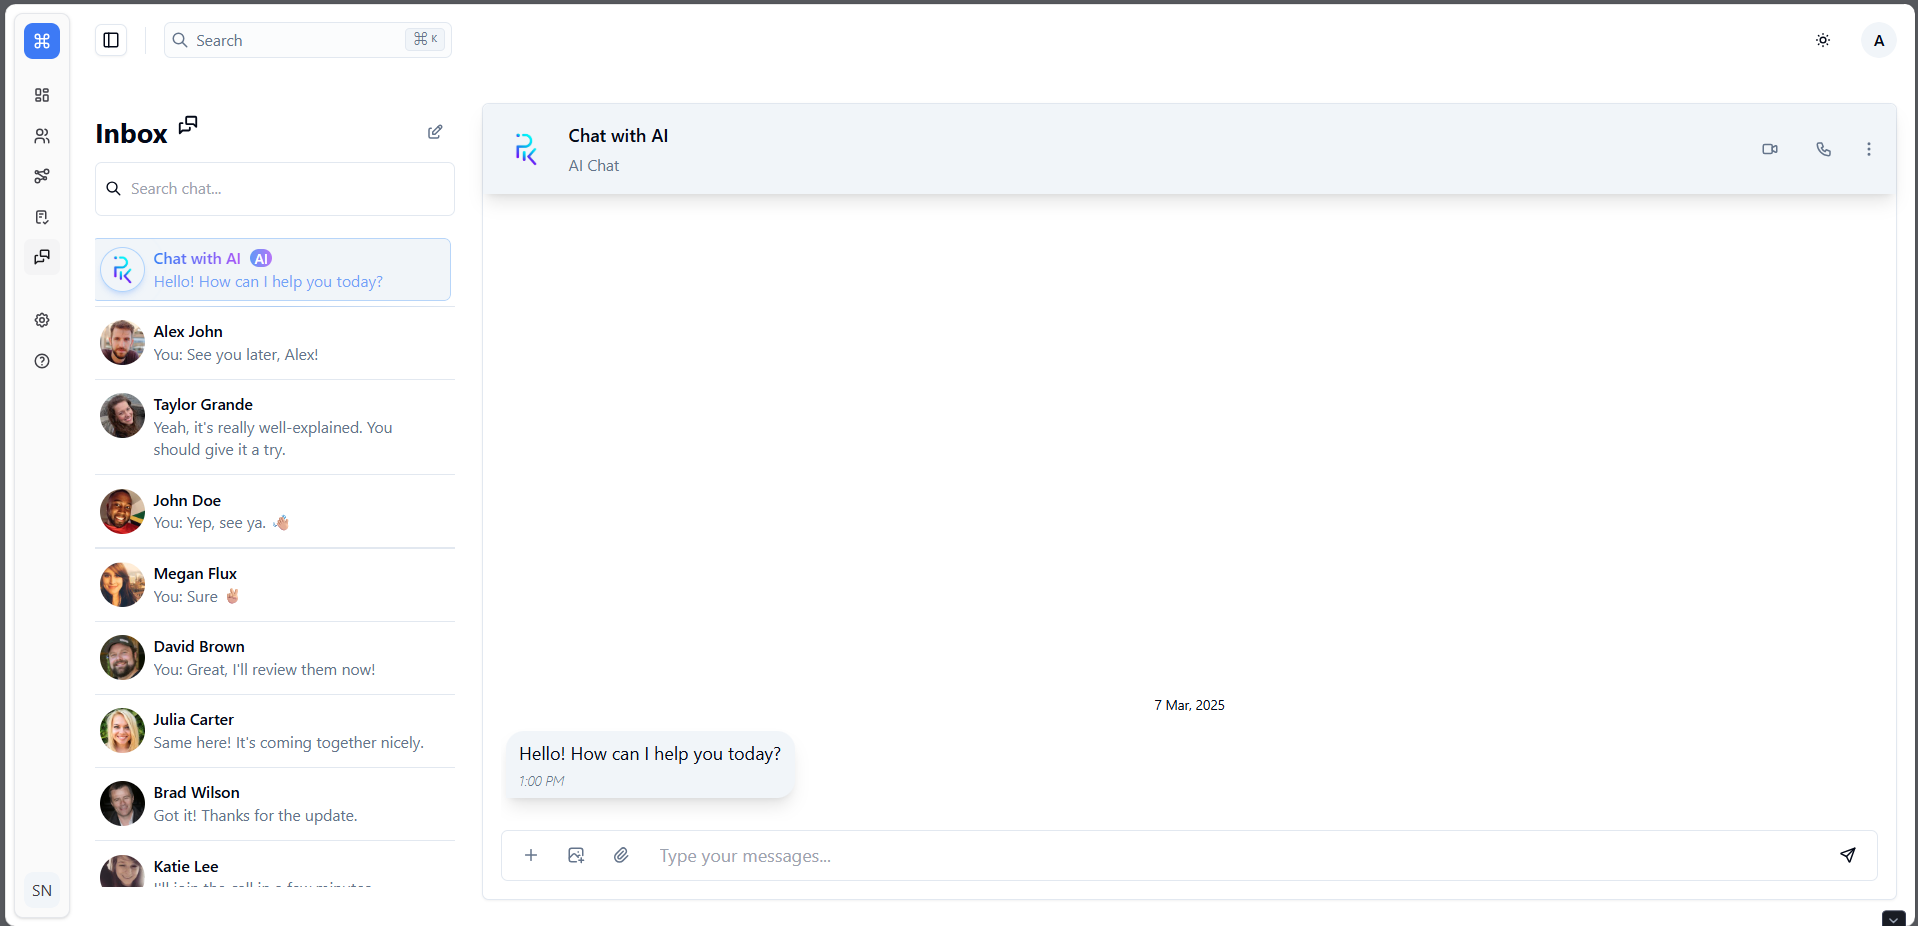
\includegraphics[width=1\textwidth]{images/assistant_web_interface.png}
    \caption{Web Interface for Real Estate Assistant}
    \label{fig:assistant-web-interface}
\end{figure}

\newpage

\subsection{Test}
\subsubsection{Test Scenarios}
The Role-Based Backoffice Agent underwent comprehensive testing across all user roles. Table \ref{tab:backoffice-test-scenarios} presents the key test scenarios.

\begin{table}[htbp]
    \centering
    \begin{tabular}{|c|l|l|l|c|}
        \hline
        \textbf{Scenario} & \textbf{User Role} & \textbf{Expected Output} & \textbf{Status} \\
        \hline
        Role identification & Super Admin & Admin dashboard access & \checkmark \\
        \hline
        Task automation & Admin & Property approval workflow & \checkmark \\
        \hline
        Performance insights & Real Estate Agent & Sales analytics & \checkmark \\
        \hline
        Permission validation & Admin & Restricted super admin features & \checkmark \\
        \hline
        AI recommendations & All roles & Role-specific suggestions & \checkmark \\
        \hline
        Workflow management & Super Admin & System optimization tips & \checkmark \\
        \hline
    \end{tabular}
    \caption{Role-Based Backoffice Agent Test Scenarios}
    \label{tab:backoffice-test-scenarios}
\end{table}

\subsection{Retrospective}

The Role-Based Backoffice Agent sprint successfully delivered customized administrative support for different user roles. Table \ref{tab:backoffice-retrospective} summarizes the key achievements and future enhancements.

\begin{table}[htbp]
    \centering
    \begin{tabular}{|p{3cm}|p{10cm}|}
        \hline
        \textbf{Category} & \textbf{Details} \\
        \hline
        \textbf{What Went Well} & 
        \begin{itemize}
            \item Successfully implemented role-based AI assistance
            \item Automated workflow management improved efficiency
            \item Web interface provides comprehensive administrative tools
            \item Role permissions and security controls work effectively
        \end{itemize} \\
        \hline
        \textbf{Action Items} & 
        \begin{itemize}
            \item Add more sophisticated automation rules
            \item Implement predictive analytics for task prioritization
            \item Enhance dashboard customization options
            \item Integrate with external business intelligence tools
        \end{itemize} \\
        \hline
    \end{tabular}
    \caption{Role-Based Backoffice Agent Sprint Retrospective Summary}
    \label{tab:backoffice-retrospective}
\end{table}

\newpage
\section{Sprint 6: Investor-Focused Recommendation System}
\subsection*{Introduction}
The Investor-Focused Recommendation System is an advanced AI model that analyzes investor behavior, preferences, and market conditions to provide personalized property investment recommendations. This system leverages machine learning algorithms to match investors with optimal investment opportunities based on their risk profile, budget, and investment goals.

\begin{figure}[htbp]
    \centering
    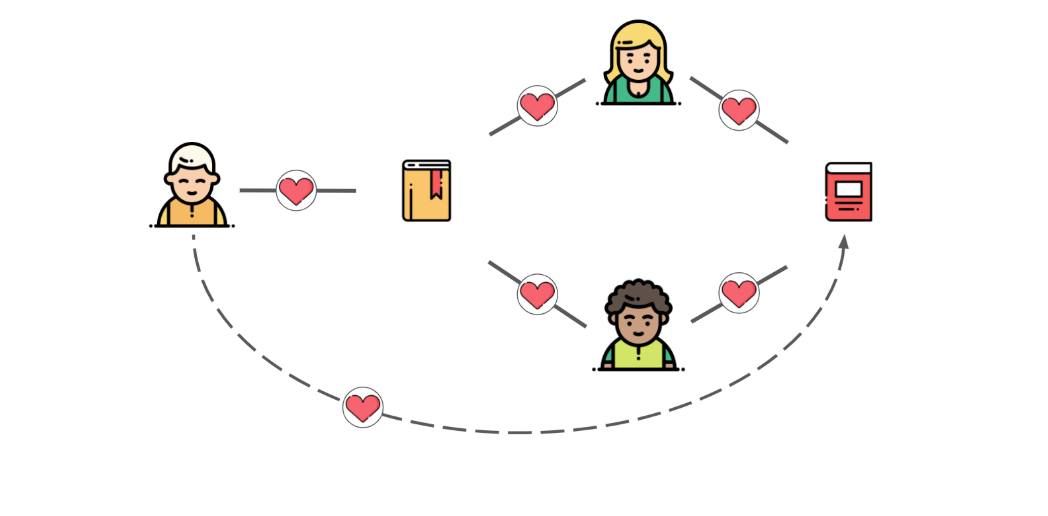
\includegraphics[width=0.7\textwidth]{images/collaborative_filtring.png}
    \caption{Collaborative Filtering Recommendation System Overview}
    \label{fig:collaborative-filtering-overview}
\end{figure}

\subsection{Analysis}
\subsubsection{Use Case Diagram}
The Recommendation System serves investors by analyzing their profiles and suggesting suitable investment opportunities. Figure \ref{fig:recommendation-use-case} illustrates the main use cases for the recommendation engine.

\begin{figure}[htbp]
    \centering
    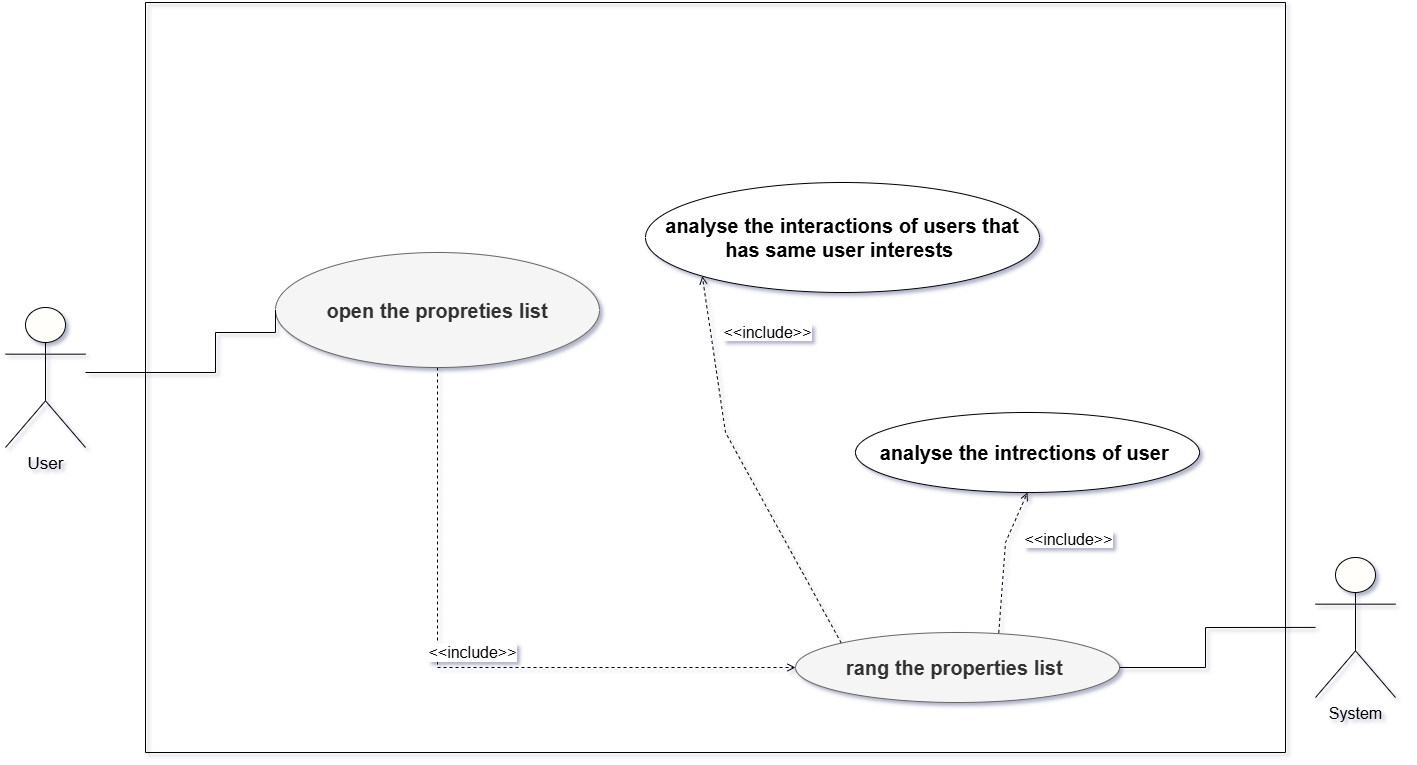
\includegraphics[width=0.7\textwidth]{images/recommendation_use_case_diagram.png}
    \caption{Investor-Focused Recommendation System Use Case Diagram}
    \label{fig:recommendation-use-case}
\end{figure}

\newpage
\subsubsection{Textual Use Case Descriptions}

\begin{table}[htbp]
    \centering
    \begin{tabular}{|p{3cm}|p{10cm}|}
        \hline
        \textbf{Use Case} & \textbf{Generate Investment Recommendations} \\
        \hline
        \textbf{Actor} & User (Investor) \\
        \hline
        \textbf{Precondition} & Investor has completed profile setup and preferences \\
        \hline
        \textbf{Main Scenario} & System matches properties with investor criteria \\
        \hline
        \textbf{Postcondition} & Investor receives tailored investment recommendations \\
        \hline
    \end{tabular}
    \caption{Investor-Focused Recommendation System Use Case Description}
    \label{tab:recommendation-use-case}
\end{table}

\subsection{Modeling}
\subsubsection{Class Diagram}
The Recommendation System uses collaborative filtering and content-based algorithms for personalized suggestions. Figure \ref{fig:recommendation-class-diagram} shows the main classes and their relationships.

\begin{figure}[htbp]
    \centering
    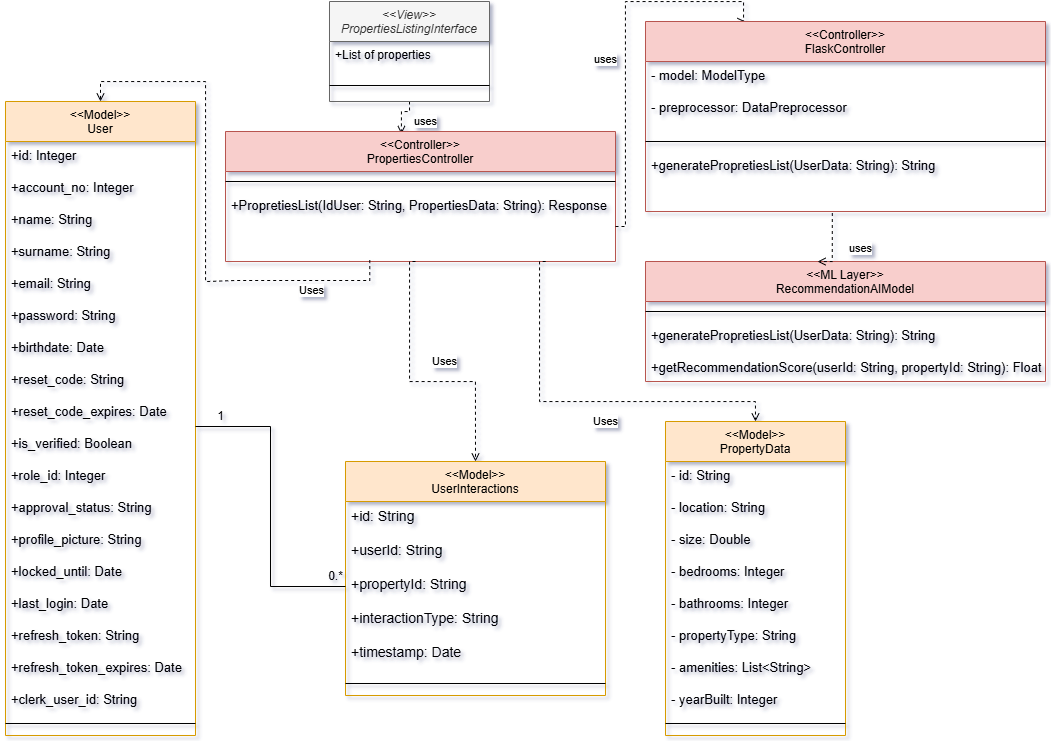
\includegraphics[width=0.8\textwidth]{images/recommendation_class_diagram.png}
    \caption{Investor-Focused Recommendation System Class Diagram}
    \label{fig:recommendation-class-diagram}
\end{figure}

\newpage
\subsubsection{Sequence Diagram (MVC)}
The interaction flow between the mobile interface, recommendation engine, and machine learning components is illustrated in Figure \ref{fig:recommendation-sequence-mvc}.

\begin{figure}[htbp]
    \centering
    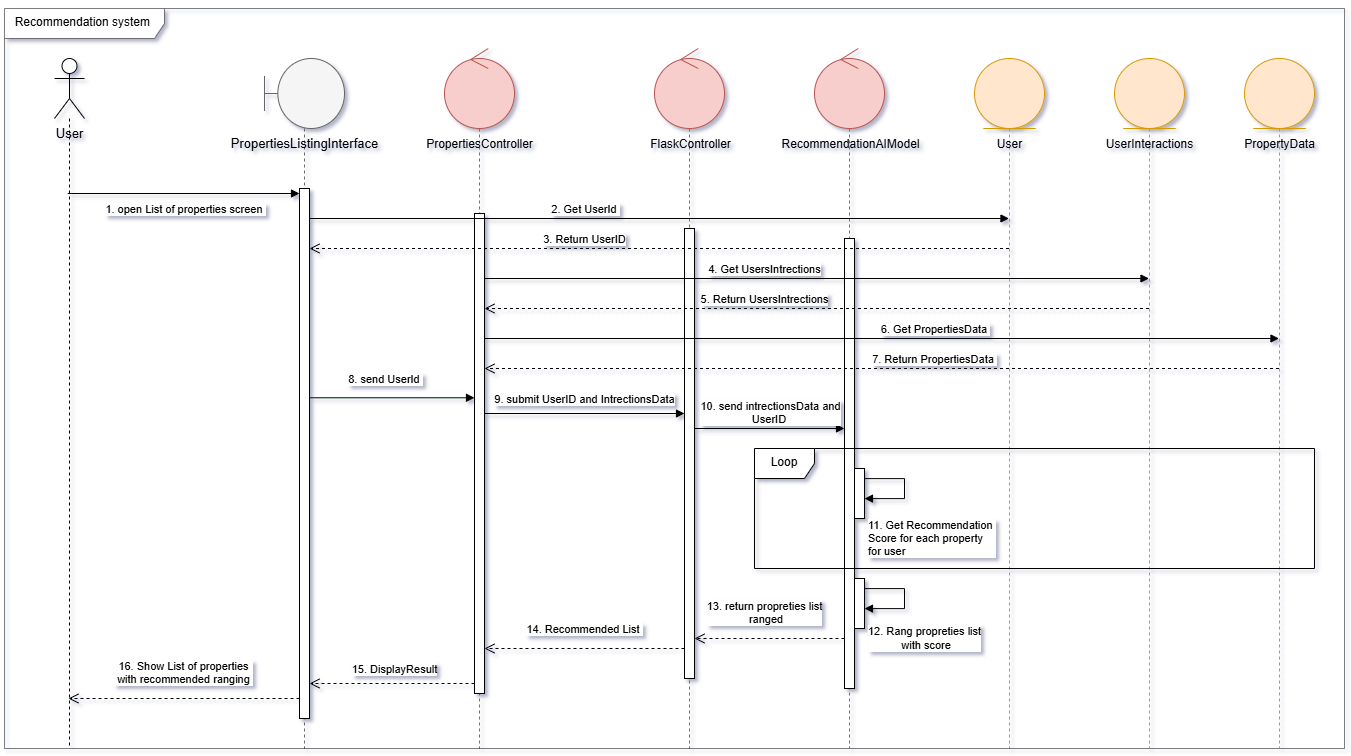
\includegraphics[width=1\textwidth]{images/recommendation_sequence_mvc.png}
    \caption{Recommendation System MVC Sequence Diagram}
    \label{fig:recommendation-sequence-mvc}
\end{figure}

\subsection{Implementation}
\subsubsection{Machine Learning Algorithms}
The Recommendation System employs multiple ML techniques for optimal suggestions:

\begin{itemize}
    \item \textbf{Collaborative Filtering}: Analyzes similar investor behaviors and preferences
    \item \textbf{Content-Based Filtering}: Matches properties based on investor criteria
    \item \textbf{Hybrid Approach}: Combines multiple algorithms for enhanced accuracy
    \item \textbf{Deep Learning}: Neural networks for complex pattern recognition
\end{itemize}


\subsubsection{Investor Profiling}
The system creates comprehensive investor profiles including:
\begin{itemize}
    \item Risk tolerance assessment
    \item Investment budget and timeline
    \item Geographic preferences
    \item Property type preferences
    \item Previous investment history
    \item Market behavior analysis
\end{itemize}

\subsubsection{Mobile Recommendations Interface}
The mobile app provides an intuitive interface for viewing personalized recommendations. Figure \ref{fig:recommendation-mobile} shows the mobile recommendation implementation.

\begin{figure}[htbp]
    \centering
    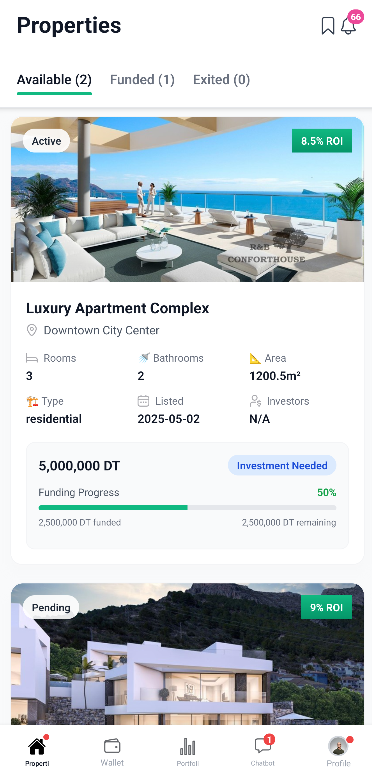
\includegraphics[width=0.3\textwidth]{images/recommendation_mobile.png}
    \caption{Mobile Interface for Investment Recommendations}
    \label{fig:recommendation-mobile}
\end{figure}

\subsubsection{Recommendation Algorithm Implementation}
The following pseudo code demonstrates our hybrid recommendation algorithm that combines user preferences, collaborative filtering, and popularity scoring:

\begin{verbatim}
FUNCTION calculate_property_score(user_id, property_id):
    user_score = get_user_preference_score(user_id, property_id)
    similar_score = get_similar_users_score(user_id, property_id)
    popularity_score = get_popularity_score(property_id)
    
    final_score = (user_score * 0.5) + (similar_score * 0.3) + (popularity_score * 0.2)
    RETURN final_score

FUNCTION get_user_preference_score(user_id, property_id):
    user = get_user(user_id)
    property = get_property(property_id)
    score = 0
    
    IF property.type == user.preferred_type: score += 30
    IF property.location == user.preferred_location: score += 20
    score += count_matching_amenities(property.amenities, user.preferred_amenities) * 2
    
    RETURN score

FUNCTION get_similar_users_score(user_id, property_id):
    similar_users = find_similar_users(user_id, limit=10)
    total_score = 0
    user_count = 0
    
    FOR each similar_user IN similar_users:
        interaction = get_user_interaction(similar_user.id, property_id)
        IF interaction exists:
            weighted_score = calculate_interaction_score(interaction) * similar_user.similarity
            total_score += weighted_score
            user_count += 1
    
    RETURN user_count > 0 ? total_score / user_count : 0

FUNCTION find_similar_users(user_id, limit):
    target_user = get_user(user_id)
    similar_users = []
    
    FOR each other_user IN get_all_users():
        IF other_user.id != user_id:
            similarity = calculate_user_similarity(target_user, other_user)
            IF similarity > 0.3:
                similar_users.add({'id': other_user.id, 'similarity': similarity})
    
    similar_users.sort_by_similarity_desc()
    RETURN similar_users.take(limit)

FUNCTION calculate_user_similarity(user1, user2):
    similarity = 0
    
    IF user1.preferred_type == user2.preferred_type: similarity += 0.3
    IF user1.preferred_location == user2.preferred_location: similarity += 0.3
    similarity += count_common_amenities(user1.amenities, user2.amenities) * 0.05
    
    RETURN min(similarity, 1.0)

FUNCTION calculate_interaction_score(interaction):
    base_scores = {"view": 10, "favorite": 30, "contact": 50, "invest": 90}
    score = base_scores[interaction.type]
    
    days_ago = days_since(interaction.timestamp)
    IF days_ago <= 7: score *= 1.2
    ELSE IF days_ago > 30: score *= 0.8
    
    RETURN score

\end{verbatim}


\subsubsection{Personalized Dashboard}
Investors receive a personalized dashboard with recommendations and portfolio insights. Figure \ref{fig:recommendation-dashboard} shows the recommendation dashboard design.


\subsection{Test}
\subsubsection{Test Scenarios}
The Recommendation System underwent extensive testing to ensure accuracy and relevance. Table \ref{tab:recommendation-test-scenarios} presents the key test scenarios.

\begin{table}[htbp]
    \centering
    \begin{tabular}{|c|l|l|l|c|}
        \hline
        \textbf{Scenario} & \textbf{Input} & \textbf{Expected Output} & \textbf{Status} \\
        \hline
        Algorithm accuracy & Historical data & High precision score & \checkmark \\
        \hline
        New investor profile & Basic preferences & Relevant recommendations & \checkmark \\
        \hline
    \end{tabular}
    \caption{Recommendation System Test Scenarios}
    \label{tab:recommendation-test-scenarios}
\end{table}

\subsubsection{Algorithm Visualization Results}
The recommendation algorithm generates personalized property rankings based on user preferences and collaborative filtering. Figure \ref{fig:recommendation-visualization} demonstrates the algorithm's output for different user profiles, showing both final scores and component breakdowns.

\newpage
\begin{figure}[htbp]
    \centering
    \begin{minipage}{0.8\textwidth}
        \centering
        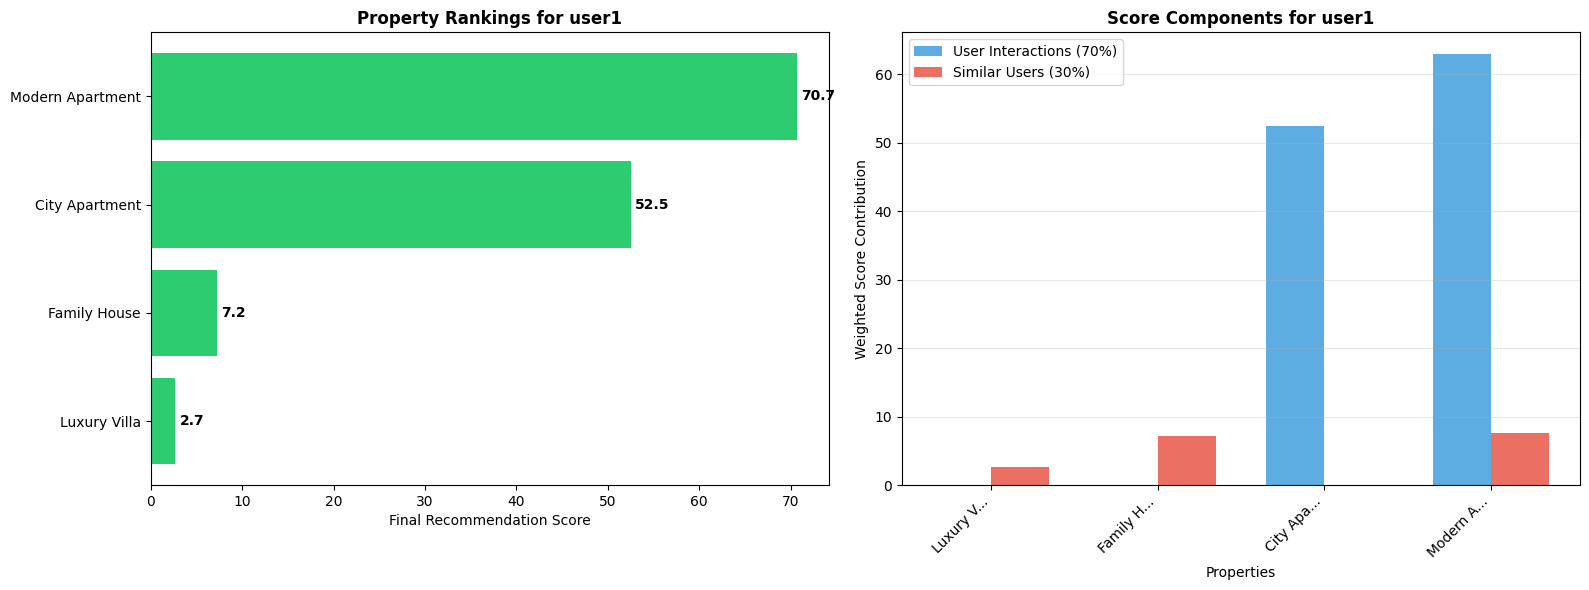
\includegraphics[width=\linewidth]{images/recommendation_user1_rankings.png}
        \caption*{Property Rankings for User1}
    \end{minipage}
    
    \begin{minipage}{0.8\textwidth}
        \centering
        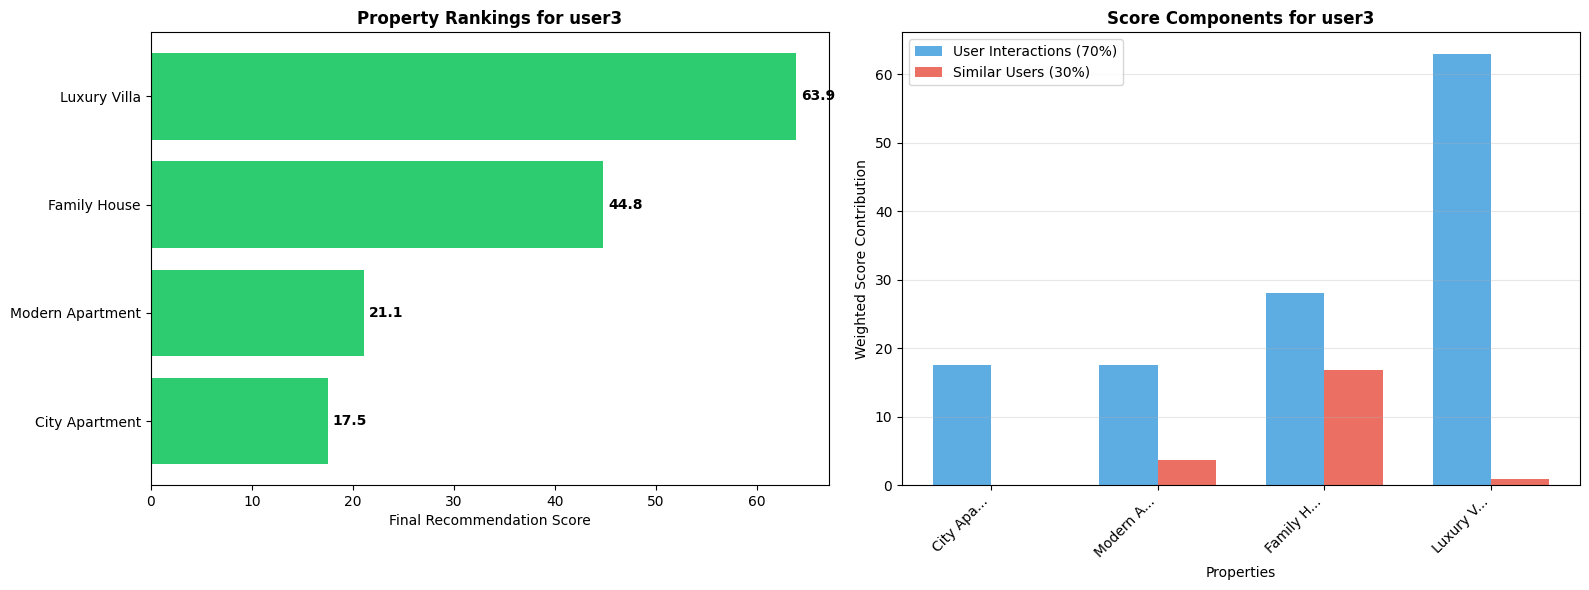
\includegraphics[width=\linewidth]{images/recommendation_user3_rankings.png}
        \caption*{Property Rankings for User3}
    \end{minipage}
    
    \caption{Recommendation Algorithm Visualization Results}
    \label{fig:recommendation-visualization}
\end{figure}

\subsection{Retrospective}

The Investor-Focused Recommendation System sprint successfully delivered personalized investment guidance through advanced machine learning algorithms. Table \ref{tab:recommendation-retrospective} summarizes the key achievements and future improvements.


\begin{table}[htbp]
    \centering
    \begin{tabular}{|p{3cm}|p{10cm}|}
        \hline
        \textbf{Category} & \textbf{Details} \\
        \hline
        \textbf{What Went Well} & 
        \begin{itemize}
            \item Successfully implemented collaborative filtering algorithms
            \item Mobile interface provides excellent user experience
            \item Comprehensive testing validated system performance
        \end{itemize} \\
        \hline
        \textbf{Action Items} & 
        \begin{itemize}
            \item Implement real-time model
        \end{itemize} \\
        \hline
    \end{tabular}
    \caption{Investor-Focused Recommendation System Sprint Retrospective Summary}
    \label{tab:recommendation-retrospective}
\end{table}




\addtocontents{toc}{\protect\newpage}

